%use scrbook and set dotted line
\documentclass[12pt,toc=chapterentrywithdots,openany]{scrbook}
%stores all imports
%use a4paper for a4 paper and size 
\usepackage[a4paper,left=30mm,right=30mm,top=30mm, bottom=30mm]{geometry}
%use german
\usepackage{german}
%silence a not relevant warning
%https://tex.stackexchange.com/questions/349473/suppress-warning-usage-of-package-fancyhdr-togetherscrbook-with-a-koma-scr
\usepackage{silence}
\WarningFilter{scrbook}{Usage of package `fancyhdr'}
%use catption for setup
\usepackage{caption}
%add prefix to the figure name
\usepackage{titletoc}
%use colorpackage to set font colors
\usepackage{xcolor}
%use fancyhdr to set the header
\usepackage{fancyhdr}
%use helvetica font
\usepackage[]{helvet}
%footnoteLink
\usepackage[hang, flushmargin]{footmisc}
%use graphicx to add images
\usepackage{graphicx}
%use inputenc to set the encoding
\usepackage[utf8]{inputenc}
%create acronym
\usepackage{acronym}
%setQuotes
\usepackage{csquotes}
%useUnicode
\usepackage{lmodern}
%useFloatLocations
\usepackage{float}
%user hyperref to add links
\usepackage{hyperref}
%define items
\usepackage{enumitem}
%useArrayTables
\usepackage{array}
\hypersetup{
    colorlinks=true,
    linkcolor=black,
    urlcolor=blue,
    citecolor=red,
}



%set the caption to the left side
\captionsetup{justification=raggedright,singlelinecheck=false}
% Verhindert, dass nur eine Zeile auf der nächsten Seite steht
\setlength{\marginparwidth}{2cm}
\usepackage[all]{nowidow}

%options for figures
%reset the counter to have no chapter numberings
\setcounter{figure}{0}
\renewcommand{\thefigure}{\arabic{figure}}


%reset the figure name
\renewcommand{\figurename}{Bild}

% Format the figure appearance in ToF
\titlecontents{figure}[0mm]%
{}%  % No extra indentation
{}%  % Format: Bild <number>:
{}%
{\titlerule*[1pc]{.}\contentspage}  % Dotted line and page number
%options for tables

%renewcommand to apply the font
\renewcommand\familydefault{\sfdefault}
\setuptoc{toc}{totoc}
%start the document
\begin{document}


%titlepage
%variableto fill
\newcommand{\Thema}{STH - Konzept und Implementierung der plattformunabhängigen SportTalentHub App für den Austausch zwischen Spieler und Sportmanager}
\newcommand{\Name}{Jonas Waigel, Fitim Makolli, Hasan Deveci und Vatsegkan Zournatsidis}
\newcommand{\Matrikelnummer}{590367, 590827, 587470 und 585568}
\newcommand{\Gutachter}{Prof. Dr. Joachim Berlak}
\newcommand{\Abgabedatum}{\today}




\begin{titlepage}
	\newgeometry{left=2cm, right=2cm, top=2cm, bottom=2cm}
	%center the logo and display the FOM graphic
	\begin{center}
		
\includegraphics[width=2.3cm]{assets/fomLogo.pdf}\\
		\vspace{.5cm}
		%strong text
		\begin{Large}\textbf{FOM Hochschule für Ökonomie und Management}\end{Large}\\
		\vspace{.5cm}
		Hochschulzentrum München

		\vspace{2cm}
	\end{center}

	%create big space
	\bigskip

	\begin{center}
		%bold text
		\textbf{Seminararbeit}\\
		\vspace{0.2cm}
		Im Rahmen des Moduls\\
		\vspace{0.5cm}
		Anwendungsprojekt\\
		\vspace{2cm}
		Über das Thema\\
		\vspace{0.5cm}
		%bold text
		\begin{Large}\textbf{\textbf{\Thema}}\end{Large}\\

		\vspace{2cm}
		von\\
		\vspace{0.5cm}
		\begin{Large}\textbf{\textbf{\Name}}\end{Large}\\
	\end{center}

	%postion in bottom left
	\begin{figure}[b]

		Gutachter: \Gutachter       \\
		Matrikelnummer: \Matrikelnummer \\
		Abgabedatum: \Abgabedatum
	\end{figure}

\end{titlepage}
%inhaltsverzeichnis
%pagenumbering
\fancypagestyle{plain}{%
	\fancyhf{} % clear all header and footer fields
	\fancyhead{} % clear all header fields
	\fancyfoot{} % clear all footer fields
	\fancyhead[C]{\textcolor{gray}\thepage} 
	\renewcommand{\headrulewidth}{0pt}
	\renewcommand{\footrulewidth}{0pt}
}
%use roman for the page number
\pagenumbering{Roman}
%set the toc to 2
\setcounter{page}{2}


%Inhaltsverzeichnis
\tableofcontents

%abbildungen
\listoffigures
\addcontentsline{toc}{chapter}{\protect\listfigurename}

\newpage
\newpage
%reset pagestyle to continue with arabic numbering
\pagestyle{plain}
%pagenumbering
\fancypagestyle{plain}{%
	\fancyhf{} % clear all header and footer fields
	\fancyhead{} % clear all header fields
	\fancyfoot{} % clear all footer fields
	\fancyhead[C]{\textcolor{gray}\thepage}
	\renewcommand{\headrulewidth}{0pt}
	\renewcommand{\footrulewidth}{0pt}
}

\pagenumbering{Roman}

\setcounter{page}{5}

\section*{\fontsize{20}{0} \selectfont Abkürzungsverzeichnis}
\begin{acronym}[]\itemsep0pt %der Parameter in Klammern sollte die längste Abkürzung sein. Damit wird der Abstand zwischen Abkürzung und Übersetzung festgelegt
	\acro{STH-App}{\textit{Sport Talent Hub App}}
	\acro{IDE}{\textit{Integrierte Entwicklungsumgebung}}
	\acro{iOS}{\textit{Internetwork Operating System}}
	\acro{LaTeX}{\textit{Lamport TeX}}
\end{acronym}
\addcontentsline{toc}{chapter}{Abkürzungsverzeichnis}
\newpage
%reset pagestyle to continue with arabic numbering
\pagestyle{plain}
%pagenumbering
\fancypagestyle{plain}{%
	\fancyhf{} % clear all header and footer fields
	\fancyhead{} % clear all header fields
	\fancyfoot{} % clear all footer fields
	\fancyhead[C]{\textcolor{gray}\thepage}
	\renewcommand{\headrulewidth}{0pt}
	\renewcommand{\footrulewidth}{0pt}
}

\pagenumbering{arabic}

% \deffootnote{1.4em}{1em}{\footnotemark}
\deffootnote{1.5em}{1em}{\makebox[1em][l]{\footnotemark}}
\renewcommand{\footnotesize}{\fontsize{10pt}{12pt}\selectfont}


\newpage

%reset pagestyle to continue with arabic numbering
\pagestyle{plain}
%pagenumbering
\fancypagestyle{plain}{%
	\fancyhf{} % clear all header and footer fields
	\fancyhead{} % clear all header fields
	\fancyfoot{} % clear all footer fields
	\fancyhead[C]{\textcolor{gray}\thepage}
	\renewcommand{\headrulewidth}{0pt}
	\renewcommand{\footrulewidth}{0pt}
}

\pagenumbering{arabic}

% \deffootnote{1.4em}{1em}{\footnotemark}
\deffootnote{1.5em}{1em}{\makebox[1em][l]{\footnotemark}}
\renewcommand{\footnotesize}{\fontsize{10pt}{12pt}\selectfont}
%start
\chapter{Kurzbeschreibung}
Diese Projektdokumentation behandelt das Konzept und die Implementierung der plattformunabhängigen STH-App für den Austausch zwischen Spielern und Sportmanagern.
Dabei werden zunächst die wichtigsten Voraussetzungen wie die Teambildung, die Projektinitiierung und die Projektskizze beschrieben.
Das Projektteam besteht aus vier Projektmitgliedern: Jonas Waigel, Fitim Makolli, Hasan Deveci und Vatsegkan Zournatsidis.
Zusätzlich hat das Team Jonas Waigel als Projektleiter gewählt.
Durch ihre einzigartigen Fähigkeiten, Erfahrungen und die gemeinsame Vision, eine innovative Smartphone-App zu gestalten, sowie ihre Leidenschaft für Sport, erlangte das Team den notwendigen Spirit und die Dynamik, um ein herausragendes Produkt zu erschaffen.
\newline
Die STH-App, kurz für „Sports Talent Hub“, wurde entwickelt, um Sportlern und Sportmanagern eine reibungslose Interaktion und Vernetzung zu bieten.
Spieler haben die Möglichkeit, ihre Profile zu erstellen, ihre sportlichen Erfolge und Höhepunkte zu teilen und mit möglichen Managern in Verbindung zu treten.
Sportmanager können gleichzeitig Talente identifizieren, kontaktieren und für unterschiedliche sportliche Projekte einstellen.
\newline
Nach vielen Recherchen und Überlegungen entwickelte das Projektteam eine Smartphone-App, die plattformunabhängig ist und den Austausch und das Anwerben zwischen Spielern und Sportmanagern ähnlich der Social Media App Instagram ermöglicht.
Die STH-App zielt darauf ab, eine Plattform zu schaffen, die effizient und benutzerfreundlich ist und Sportlern sowie Managern die Kommunikation und Zusammenarbeit in einem dynamischen und interaktiven Umfeld ermöglicht.
\newline
Das Konzept und die Umsetzung eines MVP (Minimum Viable Product) für die Anwendung sollen zwischen dem 10. März 2024 und dem 5. Juli 2024 entwickelt und in dieser Dokumentation erläutert werden.
Damit das Projekt flexibel auf Veränderungen reagieren und kontinuierliche Verbesserungen umsetzen kann, wird es agil in einer angepassten Form von Scrum durchgeführt.
Die Gründung eines Teams und eine deutliche Verteilung der Rollen innerhalb des Projekts sind für den Erfolg von großer Bedeutung.
Jeder Teilnehmer des Projekts bringt bestimmte Kompetenzen und Erfahrungen mit sich, die das gesamte Projektteam stärken.
Als Projektleiter übernimmt Jonas Waigel zusätzlich zur App-Entwicklung die Koordination der Tätigkeiten und stellt sicher, dass die Zeitpläne und Ziele eingehalten werden.
Die erfolgreiche Implementierung der App wird wesentlich von Fitim Makolli, Hasan Deveci und Vatsegkan Zournatsidis durch ihre Fachkenntnisse in den Feldern Entwicklung, Design und Qualitätssicherung beeinflusst.
\chapter{Ziele}
In diesem Kapitel werden die Muss-, Soll-, Kann- und Nicht-Ziele für das Projekt STH-App aufgezeigt.
\\

\textbf{Muss-Ziele}
\begin{itemize}
    \item Die STH-App muss als plattformunabhängige App mit einen Source-Code implementiert werden, die auf verschiedenen Betriebssystemen und Geräten implementiert (vorzugsweise macOS und Windows) und ausgeführt (vorzugsweise iOS und Android) werden kann.
    \item Die Chat-Funktion in der STH App muss es ermöglichen, eine sichere Kommunikation zwischen den App-Nutzern aufbauen zu können.
    \item Die Projektdokumentation muss bis zum 21.06.2024 vom Projektteam komplett fertiggestellt und durch die anderen Projektmitglieder Korrektur gelesen sein.
    \item Das Projektteam muss bis 15.05.2024 einen fertigen MVP incl. aller Screens in der App bereitstellen.
    \item Die STH-App für jeden Screen ein einheitliches Design aufweisen und bis zur Präsentation Design-Anpassungen und Verbesserungen durch das Projektteam durchgeführt zu haben.
\end{itemize}

\textbf{Soll-Ziele}
\begin{itemize}
    \item Die STH-App soll bis zur Abgabe der Projektarbeit am 06.07.2024 auf verschiedenen Test-Geräten und Simulatoren / Emulatoren getestet werden und Fehler als neue Aufgaben eingestellt werden.
    \item Gefundene Fehler bei App-Tests sollen bis zum 06.07.2024 durch das Projektteam gelöst werden, um das Projekt gut und mit einer funktionierenden App präsentieren zu können.
    \item Für die Veröffentlichung sollen die datenschutzrechtliche Themen und Datensicherheit durch weitere Implementierungen oder das Ausweisen wichtiger Dokumente durch das Projektteam gewährleistet sein.
\end{itemize}

\textbf{Kann-Ziele}
\begin{itemize}
    \item Nach Abschluss aller Implementierungsschritte und ausreichenden Tests kann die STH App im Apple Appstore oder Google Play Store veröffentlicht werden.
    \item Bis zu einer offiziellen App Veröffentlichung kann eine Login- und Registrierungsfunktion implementiert werden, die es ermöglicht, nutzerspezifische Inhalte zu speichern, abrufen und filtern zu können.
    \item Bei regelmäßigen Updates der App kann eine weitere Funktion für ein Hilfe- und Supportcenter angeboten werden.
\end{itemize}

\textbf{Nicht-Ziele}
\begin{itemize}
    \item Auf dem Homescreen darf es keine Möglichkeit geben, Posts oder Feeds zu kommentieren.
    \item Stories und Reels ähnlich wie bei der Social Media App Instagram sollen nicht möglich sein.
    \item Die STH App soll nicht dazu dienen, Sportmanager bewerten zu können oder Transaktionen bzw. Verträge abzuschließen sondern als Kommunikationsplattform zwischen Spieler und Sportmanager.
    \item Es dürfen keine Kosten für Spieler oder Sportmanager entstehen, um die App mit allen Funktionen nutzen zu können.
    \item Es dürfen keine laufenden Kosten wie Lizenzkosten für das Projektteam entstehen.
\end{itemize}
\chapter{Stakeholderanalyse}

Für die STH App sind Stakeholder aus verschiedenen Bereichen vorhanden.
Die Applikation erstrebt einen großen Einfluss auf die Sportindustrie und das speziell auf den Prozess des Anwerbens von neuen Fußballspielern durch Vereine in unterschiedlichen Größen.

\noindent
Deshalb ist eine Stakeholderanalyse besonders wichtig, um die verschiedenen Gruppen an Interessenten zu identifizieren und zufriedenstellen zu können.
Für die Analyse werden folgende Gruppen an Stakeholdern betrachtet: Interne-, Externe-, Community- und Technische Stakeholder.

\section{Vorgehen Stakeholderanalyse}

Die Stakeholderanalyse wurde mit einem konkreten Vorgehen erstellt.
Zuerst wurde erneut die Größe und Auswirkung der Applikation betrachtet.
Dabei ist es auch wichtig, die Zielsysteme iOS und Android nicht außer Acht zu lassen, um konkrete Benutzergruppen definieren zu können.

\noindent
Innerhalb des Projektteams wurde in einem Meeting gemeinsam festgelegt, welche Stakeholder für die STH-App in Frage kommen.
Amateursportler, Sportagenturen, Manager, Vereine und Scouts sind externe Interessensgruppen, die den Erfolg der Applikation als relevant betrachten.
Diese Gruppen an Personen haben einen direkten Bezug zur Applikation und stellen die zukünftigen Anwender dar.
Das Interesse am Verlauf und Erfolg der Applikation ist in diesen Gruppen stark vertreten, da hier ein Mehrwert für all diese Gruppen erzielt werden kann.
Aus der Hülle der Anwender heraus wurden weitere Stakeholdergruppen vom Projektteam erkannt.

\noindent
Eine weitere relevante Gruppe ist die Community hinter den Anwendern.
Dazu zählen Sportmedien und große Sportverbände, die keinen direkten Bezug zur Applikation haben, aber dennoch am Einfluss der STH-App in ihren Sportbereichen interessiert sind.
Sportmedien werden über die Bekanntmachungen von neuen Verträgen über die STH-App berichten.
Sporverbände sind an großen und performanten Sportvereinen interessiert, welche über die STH-App die Kommunikation für Spielertransfers durchführen können.

\noindent
Zu den Externen und Community Stakeholdern wurden zudem die technischen und rechtlichen Interessensgruppen erkannt.
Innerhalb der STH-App werden persönliche Daten wie z.B. Name, Vorname, Wohnort, PLZ und die E-Mail hinterlegt.
Die personenbezogenen Daten unterliegen strikten Regeln durch die Gesetzgebung der Datenschutz-Grundverordnung.
Datenschutzbeauftragte werden ein großes Interesse an der korrekten Datenhaltung der STH-App nach der Veröffentlichung der Anwendung haben.
Zudem sind die App-Stores wie der Google Play Store und der Apple App Store daran interessiert, dass diese Gesetzgebungen eingehalten werden und zudem auch die Richtlinien und Vorgaben der Stores eingehalten werden.
Die Applikation muss für eine Veröffentlichung auf diesen Plattformen diesen Regelungen strikt folgen.
Deshalb zählen diese Firmen und Personengruppen zu einem weiteren großen Teil der Stakeholder.

\noindent
Zuletzt wurden die internen Stakeholder betrachtet.
Dabei wurde das Projektteam und das Hochschulpersonal identifiziert.
Das Projektteam der STH-App ist am Erfolg der Applikation interessiert, da das Projektteam sowohl an der Organisation und an der Entwicklung der STH-App beteiligt ist.
Zudem ist das Hochschulpersonal inklusive dem Dozenten am Verlauf des Projektes interessiert, da es sich hierbei um einen Leistungsnachweis innerhalb des Wirtschaftsinformatikstudiums handelt.

\noindent
Die Stakeholderanalyse zeigt zum aktuellen Zeitpunkt der STH-App eine Vielzahl an Interessensgruppen auf, die am Erfolg oder an dem Verlauf des Projektes STH-App interessiert sind.


\section{Grafische Darstellung Stakeholderanalyse}

In der folgenden Abbildung sind die Stakeholdergruppen und deren Abhängigkeiten aufgezeichnet.
\begin{figure}[H]
	\setcounter{figure}{4} 
	\caption[Stakeholderanalyse]{Stakeholderanalyse}
	\centering
	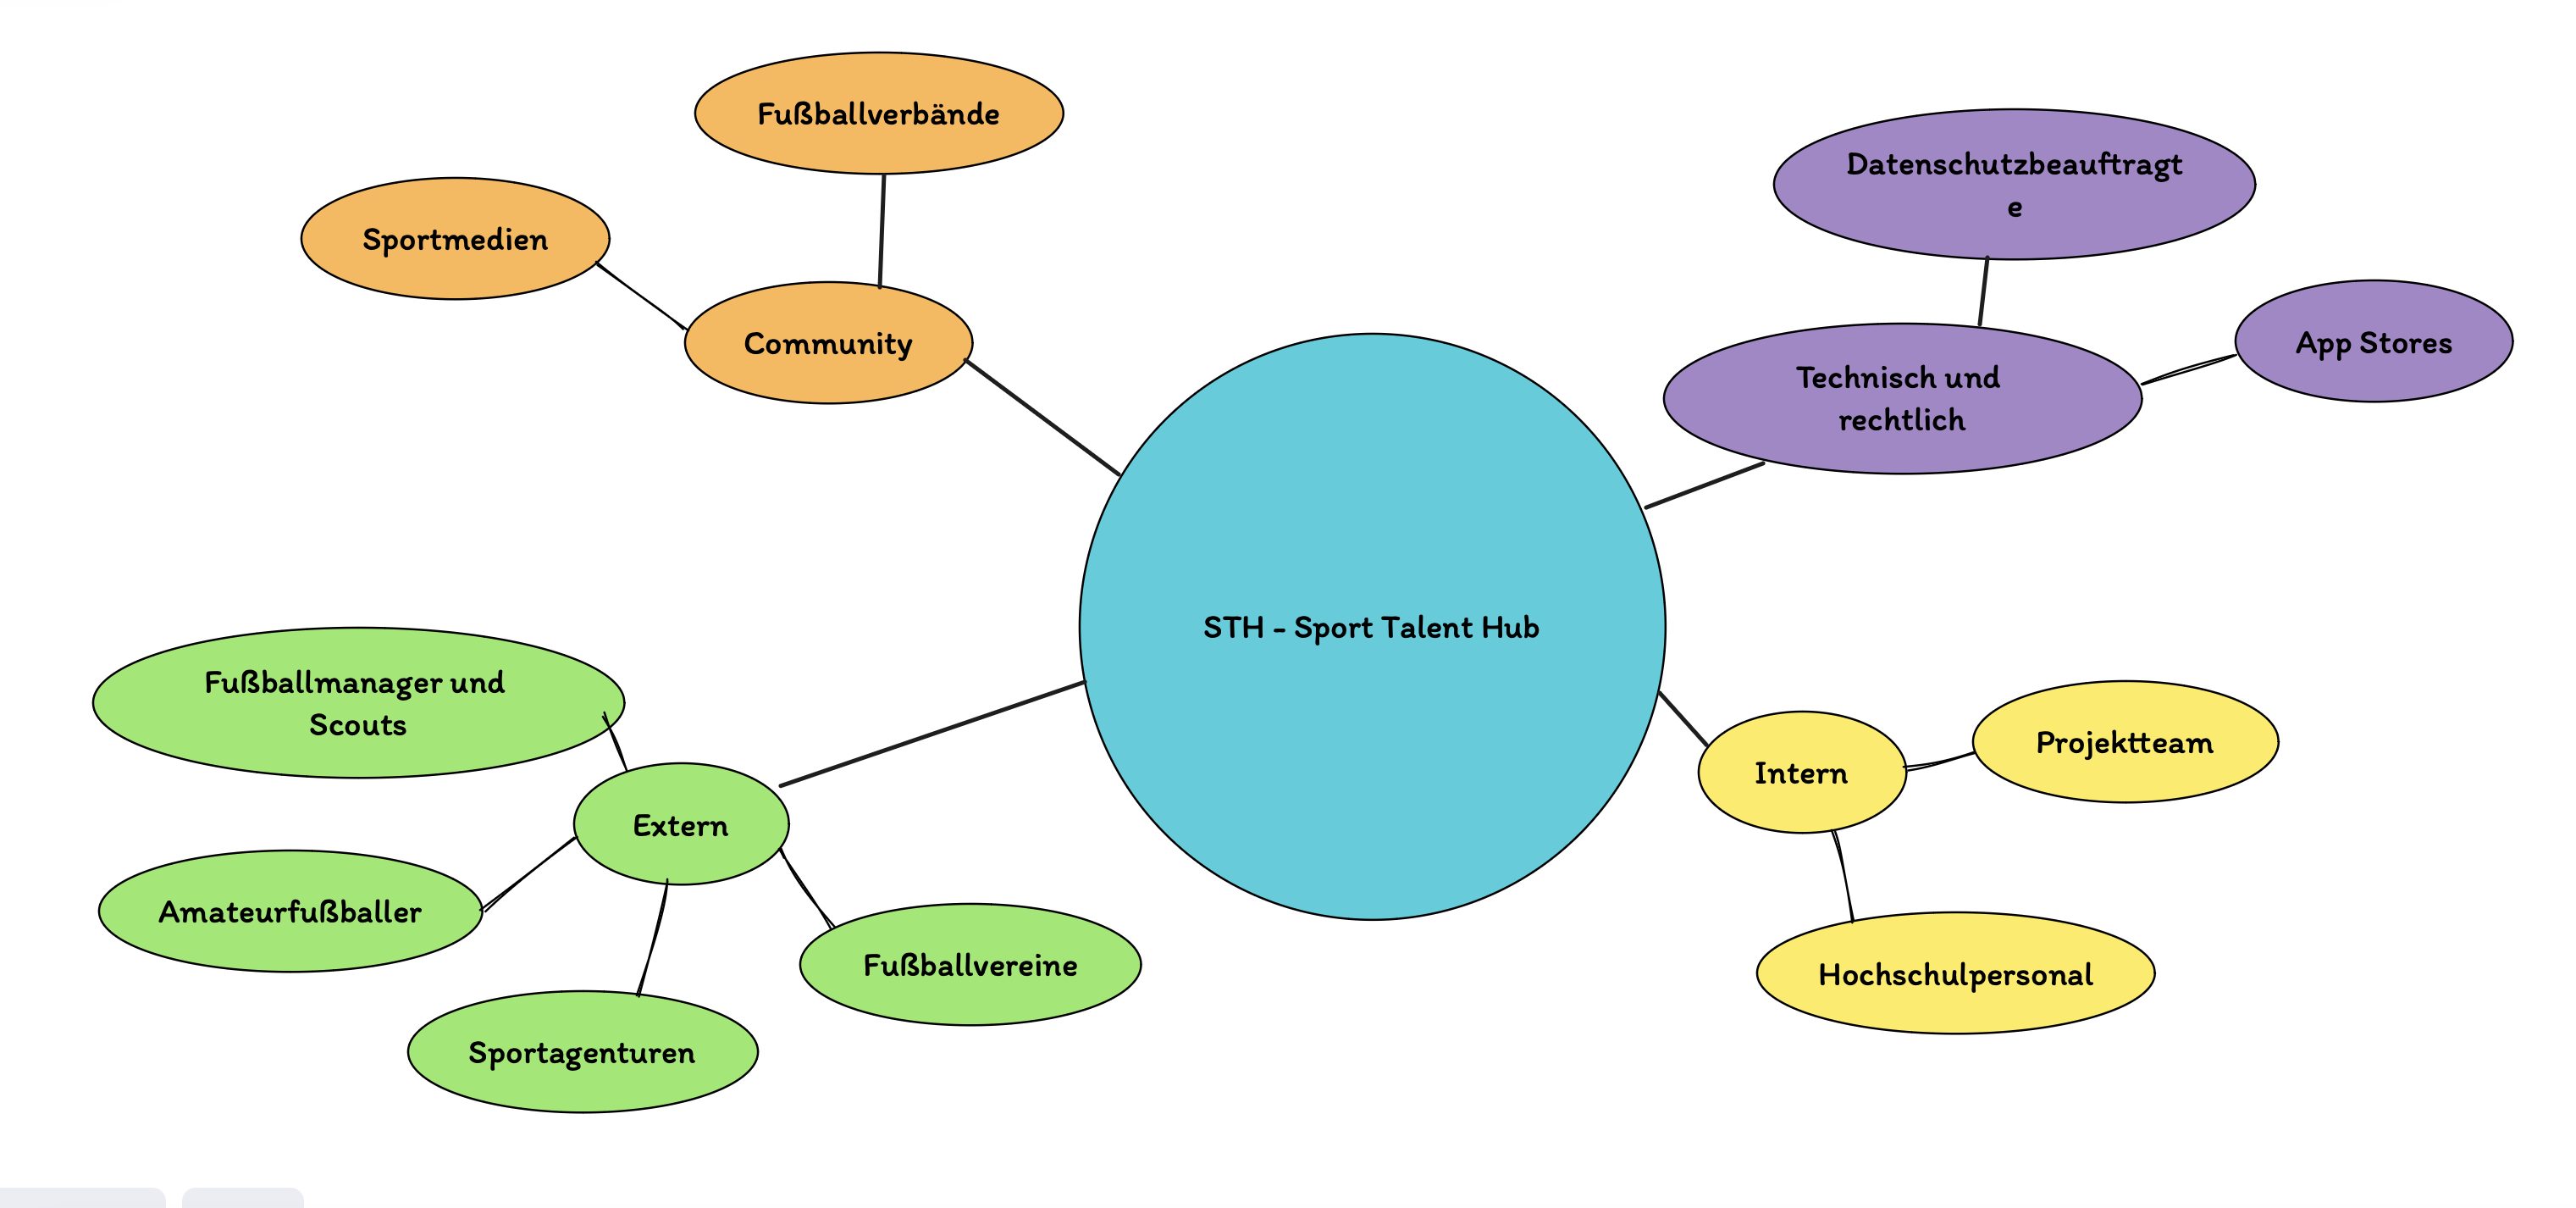
\includegraphics[width=0.9\textwidth]{assets/figures/Stakeholderanalyse.png}
	\begin{flushleft}
		Quelle: Eigene Darstellung
	\end{flushleft}
\end{figure}



\chapter{Risikoanalyse}

Die Risikoanalyse dient dazu kritische Einflüsse innerhalb und außerhalb des Projektes zu identifizieren. Für die STH App gilt vergleichbar zu allen anderen Projekten, dass der Projekterfolg nur mit begleitenden Risiken ermöglicht werden kann. Für die Klassifizierung und Einschätzungen der Risiken dient eine Risikomatrix. Hierbei wird aufgezeigt welche Risiken mit welcher Eintrittswahrscheinlichkeit und zugehöriger Auswirkung eintreten können. Anhand dessen kann bewertet werden, welche Risiken besonders laufend beobachtet werden müssen und ob es Risiken gibt, die den Projekterfolg maßgeblich gefährden.

\section{Vorgehen Risikoanalyse}
Um eine Risikobewertungsmatrix erstellen und veranschaulichen zu können benötigt es einige Schritte. Zunächst müssen die Risiken erkannt werden, die im Projekt auftreten können. Dabei werden sowohl interne als auch externe Faktoren beleuchtet. Zu den internen Risiken gehören z.B. Konflikte im Team und zu den externen Server Ausfallzeiten beim externen Dienstleister. Hierbei ist zu beachten, dass mit jedem vorangegangenen Projektfortschritt auch Risiken hinzukommen können. Daraufhin werden die Risiken nach ihrer Eintrittswahrscheinlichkeit klassifiziert. Die Einordnung hilft dabei Risiken zu priorisieren. Dabei werden Risiken mit hohen Eintrittswahrscheinlichkeiten genauer betrachtet und in Zukunft im Blick behalten. Zuletzt werden die Risiken nach ihrer Auswirkung eingestuft. Risiken mit hoher Eintrittswahrscheinlichkeit und hohen Auswirkungen können hierbei zum scheitern des Projektes bzw. zum Nichterfolg führen. Deshalb ist es besonders wichtig diese Art von Risiken nicht nur zu beobachten, sondern kontinuierlich zu messen welche Folgen der Eintritt haben kann.


\section{Graphische Darstellung Risikobewertungsmatrix}
Die Risikobewertungsmatrix für das Projekt STH App ist in der folgenden Abbildung (Nr einfügen) zu sehen.

\begin{figure}
	\caption[Risikomatrix]{Risikomatrix}
	\centering
	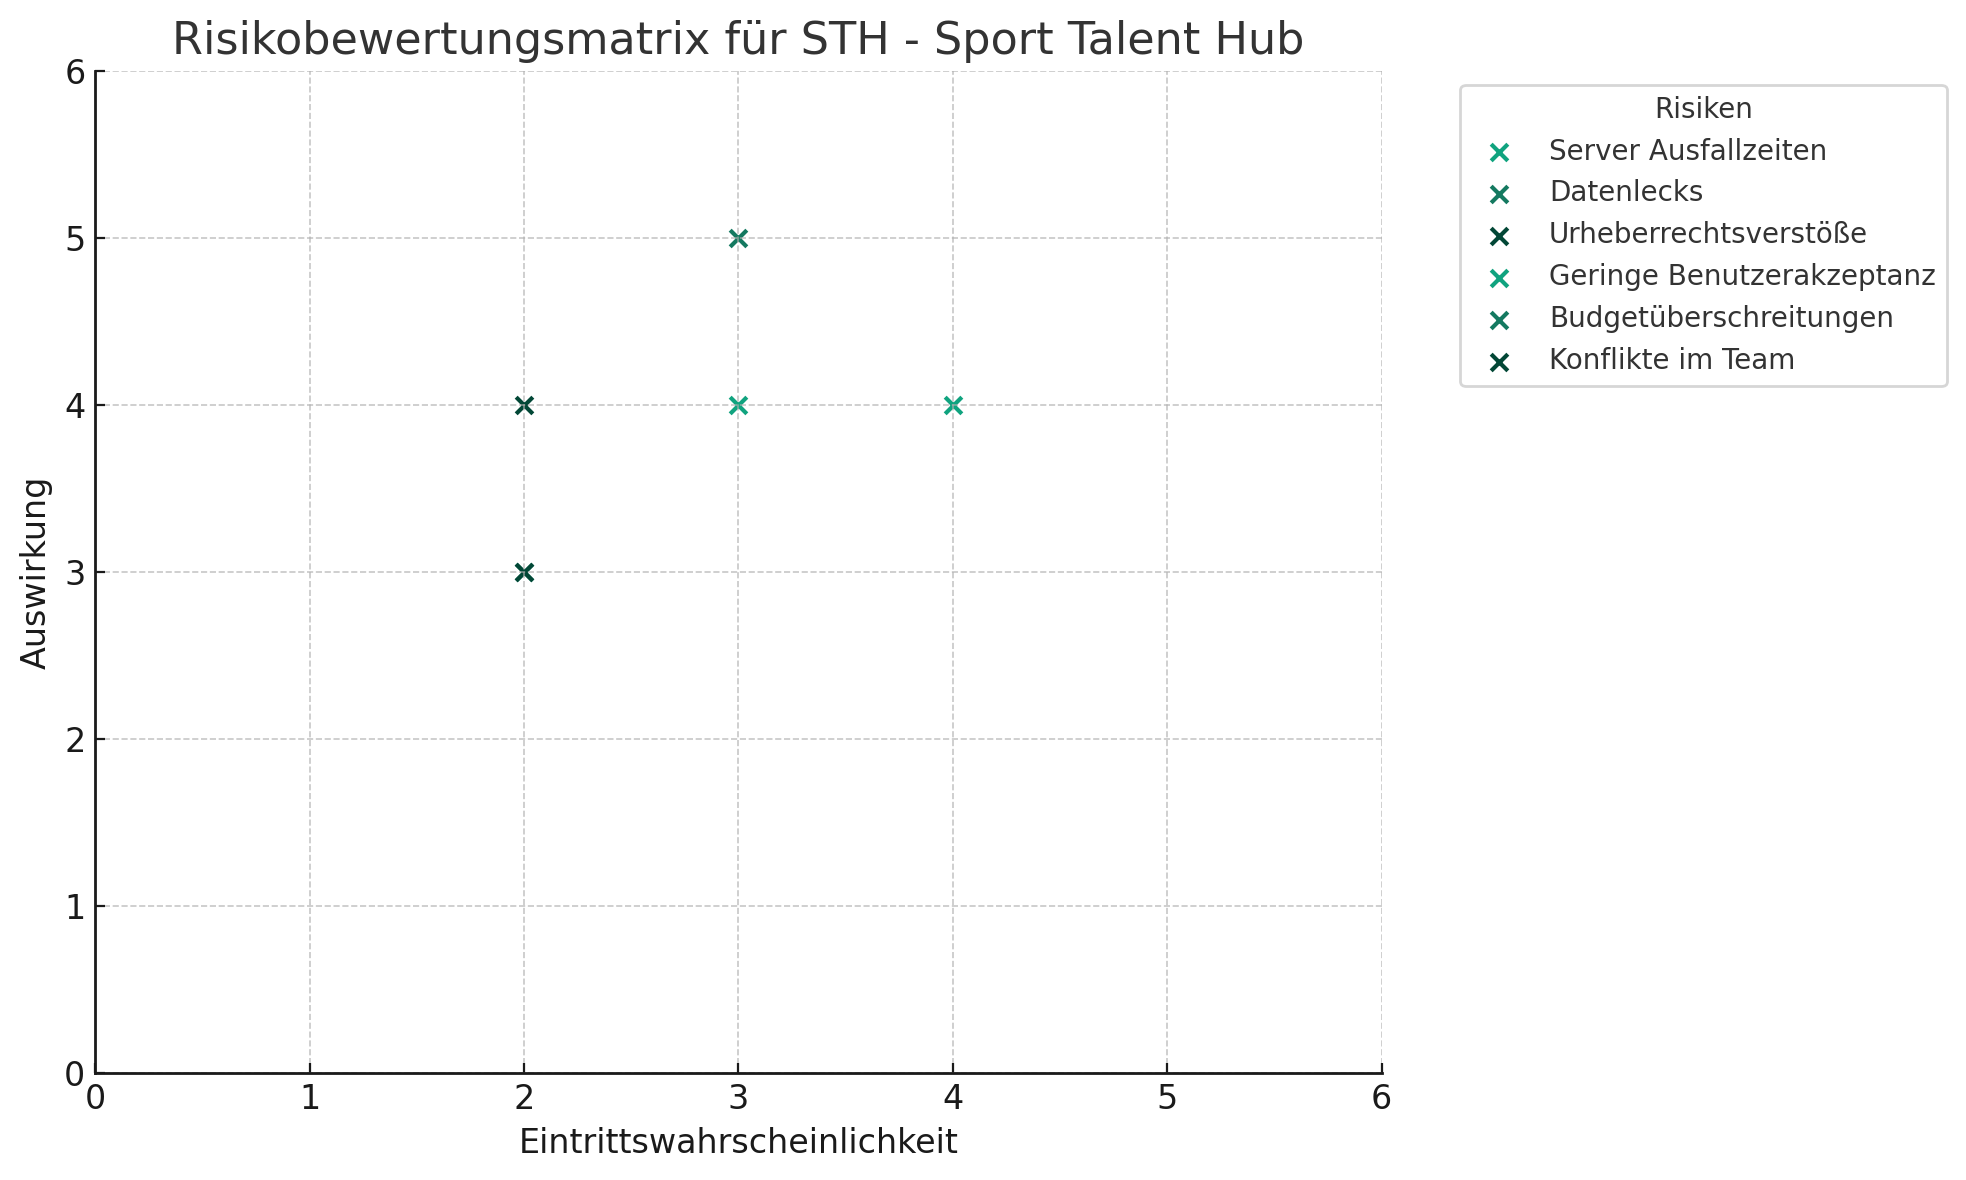
\includegraphics[width=\textwidth]{assets/figures/risikomatrix.png}
    \begin{flushleft}
		Quelle: Quelle Risikomatrix
	\end{flushleft}
\end{figure}

Für eine App mit diversen online Funktionen ist ein Server Ausfall fatal. Deshalb wurde dieses Risiko als eines der mit am höchsten verbunden Auswirkungen klassifiziert. Die Eintrittswahrscheinlichkeit bewegt sich hierbei im mittleren Bereich, da nach dem aktuellen Stand der Technik und der Rahmenverträge mit Dienstleistern bzw. Rechenzentrenten bei einem Ausfall meist auf eine redundante Serverlandschaft ausgewichen werden kann. Ein Datenleck, welches durch einen Angriff auf die Backendsysteme entstehen kann, ist für den Erfolg und gleichzeitig für die Auswirkungen einer Smartphone-App schwerwiegend. Innerhalb der STH App können sensible Daten eingegeben und abgespeichert werden, welche nicht an außenstehende gelangen dürfen. Zudem sind die immensen Kosten bezüglich der Vertragsstrafen bei der Nichteinhaltung der DSGVO ein großes finanzielles Risiko. Ein weiteres Risiko für die Applikation sind Urheberrechtsverstöße. Diese können auftreten, indem Nutzer Urheberrechtsgeschützte Inhalte veröffentlichen, welche nicht Ihnen gehören. Eine Begünstigung der Urheberrechtsverstöße könnte auf die Applikation selbst zurückzuführen sein und damit finanziell intensive Vertragsstrafen auslösen. Eine geringe Benutzerakzeptanz kann durch ein vorher schlecht ausgearbeitetes UI/UX Konzept ausgelöst werden. Die Eintrittswahrscheinlichkeit ist hierbei im mittleren Bereich, da es nicht einfach ist den Nutzern ein qualitativ hochwertiges und gut durchdachtes User-Interface zu liefern. Die Auswirkung liegt hierbei ebenso im mittleren Bereich, da das Design schnell angepasst werden kann. Die Budgetüberschreitung ist wie in fast jedem Projekt ein potenzielles Risiko, welches durchaus durch eine schlechte Planung auftreten kann. Sobald die finanziellen Ressourcen ausgeschöpft sind, kann nicht mehr an der Applikation gearbeitet und weiterentwickelt werden. Das könnte unter Umständen zu einem frühzeitigen scheitern des Projektes führen. In jedem Projektteam ist immer ein gewisses Konfliktpotenzial vorhanden. Dieses Risiko kann jederzeit und vor allem in Hochphasen wie z.B. kurz vor dem Start der Veröffentlichung der Applikation, auftreten. Allerdings ist durch eine gute Projektleitung das Risiko gut einschätzbar und präventiv vermeidbar bzw. zu lösen.



\newpage
\chapter{Produktanforderungen und technische Architektur}

In diesem Kapitel werfen wir einen umfassenden Blick auf die Produktanforderungen und die technische Architektur der STH-App.
Die STH-App bietet weit mehr als nur das Teilen von Inhalten. Sie fungiert als Social-Media-Plattform, auf der Sportmanager und Sportler miteinander kommunizieren und Fähigkeiten sowie personenbezogene Profildaten teilen können. Daher ist es von entscheidender Bedeutung, dass die Produktanforderungen einzelner Funktionen und Features separat zur Implementierung bereitgestellt werden, um den unterschiedlichen Anforderungen und Erwartungen beider Gruppen gerecht zu werden.
Genau genommen wird die STH-App eine Vielzahl von Funktionen bieten, mit denen Benutzer ihre sportlichen Ziele verfolgen und sich dabei mit anderen Benutzern vernetzen können.
Die Hauptbildschirme der STH-App, wie beispielsweise der Home-Screen, Chat-Screen, Search-Screen, Profile-Screen und der Loading-Screen, sind interaktive Schnittstellen, die die Sporterfahrung sowohl für Manager als auch für Sportler bereichern.
Der Home-Screen der STH-App bietet einen umfassenden Überblick über die sportlichen Aktivitäten und Leistungen durch die Profilanlagen der jeweiligen Benutzer. Auf diese Weise können Manager beispielsweise die Profile ihrer Athleten verfolgen und die darin enthaltenen Daten begutachten. Gleichzeitig ermöglicht er den Benutzern, ihre Ziele zu setzen, ihre Fähigkeiten zur Schau zu stellen und sich mit anderen Athleten zu vernetzen.
Der Chat-Screen hingegen bietet für Sportmanager und Athleten einen zentralen Bereich für den direkten Austausch von Textnachrichten über Chatkanäle. Dies ermöglicht eine reibungslose Kommunikation und Zusammenarbeit, indem wichtige Informationen schnell und effizient ausgetauscht werden können, um die gemeinsamen Vereinbarungen und Ziele zu erreichen.
Auf dem Search-Screen können Benutzer nach spezifischen personenbezogenen Daten oder Hashtags suchen. So wird beispielsweise das Auffinden neuer Benutzer oder das Suchen nach individuellen Informationen erleichtert, die den eigenen Interessen entsprechen.
Beim Profile-Screen können Benutzer die digitale Visitenkarte eines jeden Sportlers oder Managers einsehen. Diese enthält personenbezogene Daten sowie eine Beschreibung der Person, Bilder, Videos und Qualifikationen und ermöglicht es den Benutzern, sich ein umfassendes Bild von anderen Nutzern zu machen und potenzielle Verbindungen zu knüpfen oder Zusammenarbeit zu erleichtern.
Die Leistung der STH-App spielt eine ebenso wichtige Rolle, um sicherzustellen, dass die Benutzer ein reibungsloses Erlebnis genießen können. Dabei erfordert es eine effiziente Programmierung und Optimierung sowohl auf dem Frontend als auch auf dem Backend der App. Der Loading-Screen unterstützt dabei, sämtliche Initialisierungsfeatures der STH-App aufzurufen und damit alle verbundenen Services zu starten und zu Initialisieren.
Neben den Produktanforderungen ist auch die technische Architektur der App von entscheidender Bedeutung. Hierbei spielt die technische Architektur einer App eine entscheidende Rolle, da sie die Grundlage für Effizienz und Skalierbarkeit bildet.
Ein sorgfältig ausgewähltes Set von Technologien und Plattformen ist daher unerlässlich, um sicherzustellen, dass die Anwendung nicht nur reibungslos funktioniert, sondern auch die sich ständig wandelnden Anforderungen der Benutzer erfüllen kann.
Als Entwicklungsplattform dient Visual Studio Code, eine leistungsstarke IDE, die speziell für die Entwicklung von Flutter-Apps optimiert ist. Visual Studio Code bietet eine Fülle von Funktionen und Erweiterungen, die den Entwicklungsprozess beschleunigen und vereinfachen.
Um mit der Entwicklung in Flutter plattformunabhängig zu gestalten, ist es neben Visual Studio Code und dem Flutter-Framework wichtig, auch Android Studio zu installieren. Dies gewährleistet, dass Entwickler sowohl für iOS als auch für Android entwickeln können. Während das Flutter-Framework eine benutzerfreundliche Umgebung und eine Vielzahl von Smartphone-Emulatoren für die Entwicklung von Flutter-Apps bietet, ist Android Studio unverzichtbar für die spezifische Entwicklung von Android-Apps. Durch die Kombination beider Komponenten können Entwickler effizient und reibungslos plattformübergreifend arbeiten und damit sicherstellen, dass ihre Anwendungen auf verschiedenen Geräten und Betriebssystemen laufzeitfähig initialisiert werden können.
Darüber hinaus ist die Verwendung von Visual Studio Code in Kombination mit Basic-Miktex und Strawberry-Perl für die Erstellung von LaTeX-Dokumenten von entscheidender Bedeutung. Diese Tools ermöglichen nicht nur eine effiziente Bearbeitung und Kompilierung von LaTeX-Dokumenten, sondern auch eine reibungslose Integration dank des Docker-Add-Ons, das eine containerisierte Entwicklungsumgebung bereitstellt. Das Addon ermöglicht in diesem Zusammenhang eine verbesserte Portabilität und Konsistenz des LaTeX-Entwicklungsprozesses für die Dokumentation.
Für die Versionskontrolle und Zusammenarbeit wird auf GitHub gesetzt, eine führende Plattform für die Zusammenarbeit an Softwareprojekten. Hier können Entwickler gemeinsam am Code arbeiten, Änderungen verfolgen und Projekte dokumentieren.
Die klare Definition der Produktanforderungen sowie die Festlegung der Arbeitspakete über GitHub-Commits, in denen die Aufgabenstellung detailliert beschrieben wird, bilden zusammen mit der soliden technischen Architektur das Fundament für eine effektive Zusammenarbeit in der Entwicklung und Dokumentation des Projekts.
Flutter selbst fungiert als Cross-Platform-Framework für die Entwicklung sowohl des Frontends als auch des Backends der STH-App. Die Verwendung von Flutter bietet eine Reihe von Vorteilen, darunter eine hohe Leistung, schnelle Entwicklung und einfache Wartung.
Für das Backend der STH-App wird Firebase genutzt, eine Plattform von Google, die eine breite Palette von Diensten für die Entwicklung von Web- und Mobile-Apps bietet. Mit Funktionen wie Echtzeitdatenbanken, Authentifizierungsdiensten und Cloud-Speicher bietet Firebase eine robuste Lösung für die Anforderungen der STH-App.

\chapter{Teilprojekte und Arbeitspakete}
In diesem Kapitel liegt der Fokus auf den Arbeitspaketen, die für die Entwicklung der STH-App von entscheidender Bedeutung sind. Es wird zunächst erläutert, welche Aufgabenstellung jedes Arbeitspaket initialisiert, wobei sowohl die Verantwortlichen des Arbeitspakets als auch die damit verbundenen Ressourcen betrachtet werden.
\\
\\
\\
\textbf{Definition der Arbeitspakete:} \\

\textbf{Arbeitspaket 1 vom 08.03.2024 bis 11.03.2024}
\begin{itemize}[itemsep=0pt]
    \item{Bezeichnung: Initial Setup Flutter} 
    \item{Verantwortliche/r: Das Team} 
    \item{Ressourcen: VS Code, Flutter SDK, Android Emulator / iOS Simulator} 
    \item{Aufgabenstellung: Einrichtung der Entwicklungsumgebung für Flutter}
\end{itemize} 

\textbf{Arbeitspaket 2 vom 08.03.2024 bis 11.03.2024}
\begin{itemize}[itemsep=0pt]
    \item{Bezeichnung: Initial Setup LaTeX} 
	\item{Verantwortliche/r: Das Team} 
	\item{Ressourcen: VS Code incl\. LaTeX-Plugins, Container-Plattform (Docker)} 
	\item{Aufgabenstellung: Einrichtung der Entwicklungsumgebung für LaTeX}
\end{itemize}

\textbf{Arbeitspaket 3 vom 08.03.2024 bis 11.03.2024}
\begin{itemize}[itemsep=0pt]
    \item{Bezeichnung: Initial Setup GitHub} 
	\item{Verantwortliche/r: Das Team} 
	\item{Ressourcen: Git-Client, GitHub-Konto} 
	\item{Aufgabenstellung: Erstellung des Repositories auf GitHub}
\end{itemize}

\textbf{Arbeitspaket 4 vom 13.03.2024 bis 14.03.2024}
\begin{itemize}[itemsep=0pt]
    \item{Bezeichnung: Project Roadmap} 
	\item{Verantwortliche/r: Das Team} 
	\item{Ressourcen: Brainstorming} 
	\item{Aufgabenstellung: Definition der App Funktionalitäten}
\end{itemize} 

\newpage
\textbf{Arbeitspaket 5 vom 14.03.2024 bis 15.03.2024}
\begin{itemize}[itemsep=0pt]
    \item{Bezeichnung: Project Structure} 
	\item{Verantwortliche/r: Herr Jonas Waigel} 
	\item{Ressourcen: VS Code, Flutter Framework} 
    \item{Aufgabenstellung: Erstellung der ersten Projektstruktur in Visual Studio Code / Flutter}
\end{itemize}

\textbf{Arbeitspaket 6 vom 16.03.2024 bis 23.03.2024}
\begin{itemize}[itemsep=0pt]
    \item{Bezeichnung: Home Screen} 
	\item{Verantwortliche/r: Herr Jonas Waigel} 
	\item{Ressourcen: VS Code, Flutter Framework} 
    \item{Aufgabenstellung: Implementierung des Home-Screens incl\. Menüleiste (Bottom Navigationbar) am unteren Bildschirmrand und App Bar am oberen Bildschirmrand}
\end{itemize}

\textbf{Arbeitspaket 7 vom 18.03.2024 bis 01.04.2024}
\begin{itemize}[itemsep=0pt]
    \item{Bezeichnung: Chat Screen} 
	\item{Verantwortliche/r: Herr Hasan Deveci} 
	\item{Ressourcen: VS Code, Flutter Framework} 
    \item{Aufgabenstellung: Implementierung des Chat-Screens}
\end{itemize} 

\textbf{Arbeitspaket 8 vom 21.03.2024 bis 04.04.2024}
\begin{itemize}[itemsep=0pt]
    \item{Bezeichnung: Account Profile} 
	\item{Verantwortliche/r: Herr Fitim Makolli} 
	\item{Ressourcen: VS Code, Flutter Framework} 
    \item{Aufgabenstellung: Implementierung des Account-Profile-Screens inklusive Avatar und personenbezogene Daten}
\end{itemize}


\textbf{Arbeitspaket 9 vom 23.03.2024 bis 06.04.2024}
\begin{itemize}[itemsep=0pt]
    \item{Bezeichnung: Search Screen} 
	\item{Verantwortliche/r: Herr Vatsegkan Zournatsidis} 
	\item{Ressourcen: VS Code, Flutter Framework} 
    \item{Aufgabenstellung: Initiale Implementierung des Search-Screens}
\end{itemize}

\textbf{Arbeitspaket 10 vom 23.03.2024 bis 31.03.2024}
\begin{itemize}[itemsep=0pt]
    \item{Bezeichnung: Global Menu Bar} 
	\item{Verantwortliche/r: Herr Jonas Waigel} 
	\item{Ressourcen: VS Code, Flutter Framework} 
    \item{Aufgabenstellung: Implementierung einer globalen Menüleiste am unteren Bildschirmrand für alle Pages}
\end{itemize} 

\textbf{Arbeitspaket 11 vom 24.03.2024 bis 07.04.2024}
\begin{itemize}[itemsep=0pt]
    \item{Bezeichnung: Initial Setup Backend} 
	\item{Verantwortliche/r: Herr Jonas Waigel} 
	\item{Ressourcen: VS Code, Flutter Framework, Backend-Plattform (Firebase)}
    \item{Aufgabenstellung: Backend-Initialisierung (Firebase)}
\end{itemize}

\textbf{Arbeitspaket 12 vom 24.03.2024 bis 31.03.2024}
\begin{itemize}[itemsep=0pt]
    \item{Bezeichnung: Profile Edit Button} 
	\item{Verantwortliche/r: Herr Fitim Makolli} 
	\item{Ressourcen: VS Code, Flutter Framework} 
    \item{Aufgabenstellung: Implementierung eines Bearbeitungsbuttons für den Account-Profile-Screen}
\end{itemize}

\textbf{Arbeitspaket 13 vom 24.03.2024 bis 31.03.2024}
\begin{itemize}[itemsep=0pt]
    \item{Bezeichnung: Logo Design} 
	\item{Verantwortliche/r: Herr Vatsegkan Zournatsidis} 
	\item{Ressourcen: ChatGPT 4.0}
    \item{Aufgabenstellung: Gestaltung eines Logos für die STH-APP}
\end{itemize} 

\textbf{Arbeitspaket 14 vom 25.03.2024 bis 04.04.2024}
\begin{itemize}[itemsep=0pt]
    \item{Bezeichnung: Loading-Screen} 
	\item{Verantwortliche/r: Herr Vatsegkan Zournatsidis} 
	\item{Ressourcen: VS Code, Flutter Framework} 
    \item{Aufgabenstellung: Implementierung einer Ladebildschirm-Funktion beim Start der STH-App}
\end{itemize}

\textbf{Arbeitspaket 15 vom 27.03.2024 bis 06.04.2024}
\begin{itemize}[itemsep=0pt]
    \item{Bezeichnung: GetStream Chat} 
	\item{Verantwortliche/r: Herr Hasan Deveci} 
	\item{Ressourcen: VS Code, Flutter Framework} 
    \item{Aufgabenstellung: Implementierung von GetStream-Chat}
\end{itemize}

\textbf{Arbeitspaket 16 vom 27.03.2024 bis 28.03.2024}
\begin{itemize}[itemsep=0pt]
    \item{Bezeichnung: Chat App Bar}
	\item{Verantwortliche/r: Herr Jonas Waigel} 
	\item{Ressourcen: VS Code, Flutter Framework} 
    \item{Aufgabenstellung: Anpassung der App-Leiste auf dem Chat-Bildschirm}
\end{itemize} 

\newpage
\textbf{Arbeitspaket 17 vom 29.03.2024 bis 04.04.2024}
\begin{itemize}[itemsep=0pt]
    \item{Bezeichnung: Logo Loading-Screen} 
	\item{Verantwortliche/r: Herr Vatsegkan Zournatsidis} 
	\item{Ressourcen: VS Code, Flutter Framework} 
    \item{Aufgabenstellung: Implementierung eines Ladebildschirms mit einem Logo}
\end{itemize}

\textbf{Arbeitspaket 18 vom 31.03.2024 bis 07.04.2024}
\begin{itemize}[itemsep=0pt]
    \item{Bezeichnung: Backend Config} 
	\item{Verantwortliche/r: Herr Jonas Waigel} 
	\item{Ressourcen: VS Code, Flutter Framework, Backend-Plattform (Firebase)}
    \item{Aufgabenstellung: Implementierung der Backend-Konfiguration (Firebase), Authentifizierung und deren Methoden} 
\end{itemize}

\textbf{Arbeitspaket 19 vom 01.04.2024 bis 07.04.2024}
\begin{itemize}[itemsep=0pt]
    \item{Bezeichnung: Custom Page Routing} 
	\item{Verantwortliche/r: Herr Jonas Waigel} 
	\item{Ressourcen: VS Code, Flutter Framework} 
    \item{Aufgabenstellung: Implementierung einer benutzerdefinierten Seitenroute beim Wechsel von Pages}
\end{itemize} 

\textbf{Arbeitspaket 20 vom 02.04.2024 bis 08.04.2024}
\begin{itemize}[itemsep=0pt]
    \item{Bezeichnung: Chat UI Adjustments} 
	\item{Verantwortliche/r: Herr Hasan Deveci} 
	\item{Ressourcen: VS Code, Flutter Framework} 
    \item{Aufgabenstellung: Anpassung des Chat-Screens und der benutzerdefinierte App-Leiste}
\end{itemize}

\textbf{Arbeitspaket 21 vom 02.04.2024 bis 08.04.2024}
\begin{itemize}[itemsep=0pt]
    \item{Bezeichnung: Channel Adjustment} 
	\item{Verantwortliche/r: Herr Hasan Deveci} 
	\item{Ressourcen: VS Code, Flutter Framework} 
    \item{Aufgabenstellung: Anpassung des Chanels im Chat-Screen}
\end{itemize}

\textbf{Arbeitspaket 22 vom 02.04.2024 bis 03.04.2024}
\begin{itemize}[itemsep=0pt]
    \item{Bezeichnung: Latex Docs Update} 
	\item{Verantwortliche/r: Herr Jonas Waigel} 
	\item{Ressourcen: VS Code} 
    \item{Aufgabenstellung: Aufgabenstellung: Dokumentationsstruktur in LaTeX aktualisieren}
\end{itemize} 

\textbf{Arbeitspaket 23 vom 03.04.2024 bis 10.04.2024}
\begin{itemize}[itemsep=0pt]
    \item{Bezeichnung: Local Storage Setup} 
	\item{Verantwortliche/r: Herr Fitim Makolli} 
	\item{Ressourcen: VS Code, Flutter Framework} 
    \item{Aufgabenstellung: Implementierung eines lokalen Speichers für den Account-Profile-Screen}
\end{itemize}

\textbf{Arbeitspaket 24 vom 03.04.2024 bis 10.04.2024}
\begin{itemize}[itemsep=0pt]
    \item{Bezeichnung: Save/Load Functions} 
	\item{Verantwortliche/r: Herr Fitim Makolli} 
	\item{Ressourcen: VS Code, Flutter Framework} 
    \item{Aufgabenstellung: Implementierung einer Funktion zum Speichern/Laden für den Account-Profile-Screen}
\end{itemize}

\textbf{Arbeitspaket 25 vom 03.04.2024 bis 10.04.2024}
\begin{itemize}[itemsep=0pt]
    \item{Bezeichnung: RegEx Guidelines} 
	\item{Verantwortliche/r: Herr Fitim Makolli} 
	\item{Ressourcen: VS Code, Flutter Framework}
    \item{Aufgabenstellung: Implementierung von RegEx-Richtlinien in Bezug auf personenbezogene Daten}
\end{itemize} 

\textbf{Arbeitspaket 26 vom 03.04.2024 bis 15.04.2024}
\begin{itemize}[itemsep=0pt]
    \item{Bezeichnung: Hovering Function} 
	\item{Verantwortliche/r: Herr Fitim Makolli} 
	\item{Ressourcen: VS Code, Flutter Framework}
    \item{Aufgabenstellung: Implementierung einer Hovering-Funktion für personenbezogene Daten} 
\end{itemize}

\textbf{Arbeitspaket 27 vom 03.04.2024 bis 15.04.2024}
\begin{itemize}[itemsep=0pt]
    \item{Bezeichnung: Profile UI} 
	\item{Verantwortliche/r: Herr Fitim Makolli} 
	\item{Ressourcen: VS Code, Flutter Framework} 
    \item{Aufgabenstellung: Implementierung des Profile-Screens mit Avatar, Bilder und Mediathek}
\end{itemize}

\newpage
\textbf{Arbeitspaket 28 vom 10.04.2024 bis 18.04.2024}
\begin{itemize}[itemsep=0pt]
    \item{Bezeichnung: Media Upload} 
	\item{Verantwortliche/r: Herr Fitim Makolli} 
	\item{Ressourcen: VS Code, Flutter Framework} 
    \item{Aufgabenstellung: Implementierung von Funktionen zum Auswählen und Hochladen von Bilder und Videos}
\end{itemize} 

\textbf{Arbeitspaket 29 vom 10.04.2024 bis 18.04.2024}
\begin{itemize}[itemsep=0pt]
    \item{Bezeichnung: Profile Local Storage} 
	\item{Verantwortliche/r: Herr Fitim Makolli} 
	\item{Ressourcen: VS Code, Flutter Framework} 
    \item{Aufgabenstellung: Implementierung eines lokalen Speichers für den Profile-Screen}
\end{itemize}

\textbf{Arbeitspaket 30 vom 10.04.2024 bis 18.04.2024}
\begin{itemize}[itemsep=0pt]
    \item{Bezeichnung: Profile Save/Load} 
	\item{Verantwortliche/r: Herr Fitim Makolli} 
	\item{Ressourcen: VS Code, Flutter Framework} 
    \item{Aufgabenstellung: Implementierung einer Funktion zum Speichern/ Laden für den Profile-Screen}
\end{itemize}

\textbf{Arbeitspaket 31 vom 10.04.2024 bis 11.04.2024}
\begin{itemize}[itemsep=0pt]
    \item{Bezeichnung: App Bar Navigation} 
	\item{Verantwortliche/r: Herr Jonas Waigel} 
	\item{Ressourcen: VS Code, Flutter Framework} 
    \item{Aufgabenstellung: Anpassung der App-Leiste für die Navigation und das Verhalten beim Seitenwechsel}
\end{itemize} 

\textbf{Arbeitspaket 32 vom 13.04.2024 bis 19.04.2024}
\begin{itemize}[itemsep=0pt]
    \item{Bezeichnung: Shared Preferences} 
	\item{Verantwortliche/r: Herr Jonas Waigel} 
	\item{Ressourcen: VS Code, Flutter Framework, Backend-Plattform (Firebase)}
    \item{Aufgabenstellung: Verwendung von Shared Preferences zusammen mit Firebase-Testdaten} 
\end{itemize}

\newpage
\textbf{Arbeitspaket 33 vom 14.04.2024 bis 15.04.2024}
\begin{itemize}[itemsep=0pt]
    \item{Bezeichnung: Page Linking} 
	\item{Verantwortliche/r: Herr Fitim Makolli} 
	\item{Ressourcen: VS Code, Flutter Framework} 
    \item{Aufgabenstellung: Verlinkung der Pages von Profile-Screen und Account-Profile-Screen}
\end{itemize}

\textbf{Arbeitspaket 34 vom 16.04.2024 bis 17.04.2024}
\begin{itemize}[itemsep=0pt]
    \item{Bezeichnung: Loading-Screen Update} 
	\item{Verantwortliche/r: Herr Vatsegkan Zournatsidis} 
	\item{Ressourcen: VS Code, Flutter Framework} 
    \item{Aufgabenstellung: Aktualisierung des Loadingscreens}
\end{itemize} 

\textbf{Arbeitspaket 35 vom 16.04.2024 bis 25.04.2024}
\begin{itemize}[itemsep=0pt]
    \item{Bezeichnung: Start Page Logo} 
	\item{Verantwortliche/r: Herr Vatsegkan Zournatsidis} 
	\item{Ressourcen: VS Code, Flutter Framework} 
    \item{Aufgabenstellung: Hinzufügen vom Logo auf die Startseite}
\end{itemize}

\textbf{Arbeitspaket 36 vom 21.04.2024 bis 28.04.2024}
\begin{itemize}[itemsep=0pt]
    \item{Bezeichnung: Media Button} 
	\item{Verantwortliche/r: Herr Fitim Makolli} 
	\item{Ressourcen: VS Code, Flutter Framework} 
    \item{Aufgabenstellung: Implementierung eines Buttons für das Hochladen von Bilder und Videos}
\end{itemize}

\textbf{Arbeitspaket 37 vom 21.04.2024 bis 01.05.2024}
\begin{itemize}[itemsep=0pt]
    \item{Bezeichnung: Avatar Transmission} 
	\item{Verantwortliche/r: Herr Fitim Makolli} 
	\item{Ressourcen: VS Code, Flutter Framework, Backend-Plattform (Firebase)}
    \item{Aufgabenstellung: Implementierung von Funktionen zur Übertragung vom Avatar zum Backend} 
\end{itemize} 

\textbf{Arbeitspaket 38 vom 25.04.2024 bis 05.05.2024}
\begin{itemize}[itemsep=0pt]
    \item{Bezeichnung: Media Transmission} 
	\item{Verantwortliche/r: Herr Fitim Makolli} 
	\item{Ressourcen: VS Code, Flutter Framework, Backend-Plattform (Firebase)}
    \item{Aufgabenstellung: Implementierung von Funktionen zur Übertragung von Bilder und Videos an das Backend} 
\end{itemize}


\textbf{Arbeitspaket 39 vom 27.04.2024 bis 28.04.2024}
\begin{itemize}[itemsep=0pt]
    \item{Bezeichnung: Page Navigation} 
	\item{Verantwortliche/r: Herr Jonas Waigel} 
	\item{Ressourcen: VS Code, Flutter Framework} 
    \item{Aufgabenstellung: Anpassung der Seiten-Navigation und Entfernung von Animationen beim Wechsel}
\end{itemize}

\textbf{Arbeitspaket 40 vom 28.04.2024 bis 29.04.2024}
\begin{itemize}[itemsep=0pt]
    \item{Bezeichnung: Latex Docs Update} 
	\item{Verantwortliche/r: Herr Fitim Makolli} 
	\item{Ressourcen: VS Code} 
    \item{Aufgabenstellung: Dokumentationsstruktur in Latex aktualisiert}
\end{itemize} 

\textbf{Arbeitspaket 41 vom 29.04.2024 bis 05.04.2024}
\begin{itemize}[itemsep=0pt]
    \item{Bezeichnung: Chat Routing} 
	\item{Verantwortliche/r: Herr Hasan Deveci} 
	\item{Ressourcen: VS Code, Flutter Framework} 
    \item{Aufgabenstellung: Implementierung der Seitenroute vom Chat zum Chanelscreen}
\end{itemize} 

\textbf{Arbeitspaket 42 vom 29.04.2024 bis 05.04.2024}
\begin{itemize}[itemsep=0pt]
    \item{Bezeichnung: Profile Navigation} 
	\item{Verantwortliche/r: Herr Hasan Deveci} 
	\item{Ressourcen: VS Code, Flutter Framework} 
    \item{Aufgabenstellung: Implementierung der Navigationsroute vom Chat-Screen zum Profile-Screen}
\end{itemize} 

\textbf{Arbeitspaket 43 vom 30.04.2024 bis 10.05.2024}
\begin{itemize}[itemsep=0pt]
    \item{Bezeichnung: Stream Headers} 
	\item{Verantwortliche/r: Herr Hasan Deveci} 
	\item{Ressourcen: VS Code, Flutter Framework} 
    \item{Aufgabenstellung: Implementierung des Stream-Channel-Headers}
\end{itemize} 

\textbf{Arbeitspaket 44 vom 30.04.2024 bis 10.05.2024}
\begin{itemize}[itemsep=0pt]
    \item{Bezeichnung: Username Update} 
	\item{Verantwortliche/r: Herr Fitim Makolli} 
	\item{Ressourcen: VS Code, Flutter Framework} 
    \item{Aufgabenstellung: Implementierung der Aktualisierung des Benutzernamens auf dem Profile-Screen}
\end{itemize} 

\textbf{Arbeitspaket 45 vom 30.04.2024 bis 07.05.2024}
\begin{itemize}[itemsep=0pt]
    \item{Bezeichnung: Action Button} 
	\item{Verantwortliche/r: Herr Hasan Deveci} 
	\item{Ressourcen: VS Code, Flutter Framework} 
    \item{Aufgabenstellung: Implementierung einer Aktionsschaltfläche mit Benutzerintegration}
\end{itemize} 

\textbf{Arbeitspaket 46 vom 30.04.2024 bis 07.05.2024}
\begin{itemize}[itemsep=0pt]
    \item{Bezeichnung: Test User Addition} 
	\item{Verantwortliche/r: Herr Hasan Deveci} 
	\item{Ressourcen: VS Code, Flutter Framework} 
    \item{Aufgabenstellung: Implementierung neuer Chat-User als Testdaten}
\end{itemize} 

\textbf{Arbeitspaket 47 vom 05.05.2024 bis 15.05.2024}
\begin{itemize}[itemsep=0pt]
    \item{Bezeichnung: Hashtag Implementation} 
	\item{Verantwortliche/r: Herr Fitim Makolli} 
	\item{Ressourcen: VS Code, Flutter Framework} 
    \item{Aufgabenstellung: Implementierung von Hashtags im Profile-Screen}
\end{itemize} 

\textbf{Arbeitspaket 48 vom 06.05.2024 bis 15.05.2024}
\begin{itemize}[itemsep=0pt]
    \item{Bezeichnung: Hashtag Storage} 
	\item{Verantwortliche/r: Herr Fitim Makolli} 
	\item{Ressourcen: VS Code, Flutter Framework} 
    \item{Aufgabenstellung: Implementierung eines lokalen Speichers für die Hashtags}
\end{itemize} 

\textbf{Arbeitspaket 49 vom 06.05.2024 bis 15.05.2024}
\begin{itemize}[itemsep=0pt]
    \item{Bezeichnung: Hashtag Transmission} 
	\item{Verantwortliche/r: Herr Fitim Makolli} 
	\item{Ressourcen: VS Code, Flutter Framework} 
    \item{Aufgabenstellung: Implementierung von Funktionen zur Übertragung von Hashtags an das Backend}
\end{itemize} 

\textbf{Arbeitspaket 50 vom 07.05.2024 bis 20.05.2024}
\begin{itemize}[itemsep=0pt]
    \item{Bezeichnung: Major Bug Fixes} 
	\item{Verantwortliche/r: Herr Fitim Makolli} 
	\item{Ressourcen: VS Code, Flutter Framework} 
    \item{Aufgabenstellung: Fehlerbehebungen für den Profile-Screen und Account-Profile-Screen}
\end{itemize} 

\newpage
\textbf{Arbeitspaket 51 vom 10.06.2024 bis 15.06.2024}
\begin{itemize}[itemsep=0pt]
    \item{Bezeichnung: Search-Screen: search function} 
	\item{Verantwortliche/r: Herr Fitim Makolli} 
	\item{Ressourcen: VS Code, Flutter Framework, Firebase} 
    \item{Aufgabenstellung: Implementierung der Benutzer in Firebase und Implementierung der Firebase-Funktion zum Suchen der User}
\end{itemize} 

\textbf{Arbeitspaket 52 vom 15.06.2024 bis 15.06.2024}
\begin{itemize}[itemsep=0pt]
    \item{Bezeichnung: Search-Screen: avatar icon} 
	\item{Verantwortliche/r: Herr Fitim Makolli} 
	\item{Ressourcen: VS Code, Flutter Framework, Firebase} 
    \item{Aufgabenstellung: Implementierung leerer Avatar-Icons der aufgelisteten User}
\end{itemize} 

\textbf{Arbeitspaket 53 vom 15.06.2024 bis 15.06.2024}
\begin{itemize}[itemsep=0pt]
    \item{Bezeichnung: Update homescreen with profileImages} 
	\item{Verantwortliche/r: Herr Jonas Waigel} 
	\item{Ressourcen: VS Code, Flutter Framework, Firebase} 
    \item{Aufgabenstellung: Hinzufügen von Avatarbildern aus dem Firebase Storage im Homescreen}
\end{itemize}

\textbf{Arbeitspaket 54 vom 18.06.2024 bis 18.06.2024}
\begin{itemize}[itemsep=0pt]
    \item{Bezeichnung: Update searchscreen with profileImages} 
	\item{Verantwortliche/r: Herr Jonas Waigel} 
	\item{Ressourcen: VS Code, Flutter Framework, Firebase} 
    \item{Aufgabenstellung: Hinzufügen von Avatarbildern aus dem Firebase Storage im Search-Screen}
\end{itemize}




\chapter{Meilensteinplanung}
Wir sind geil
\begin{figure}[H]
    \caption[Meilensteinplannung]{Meilensteinplannung}
    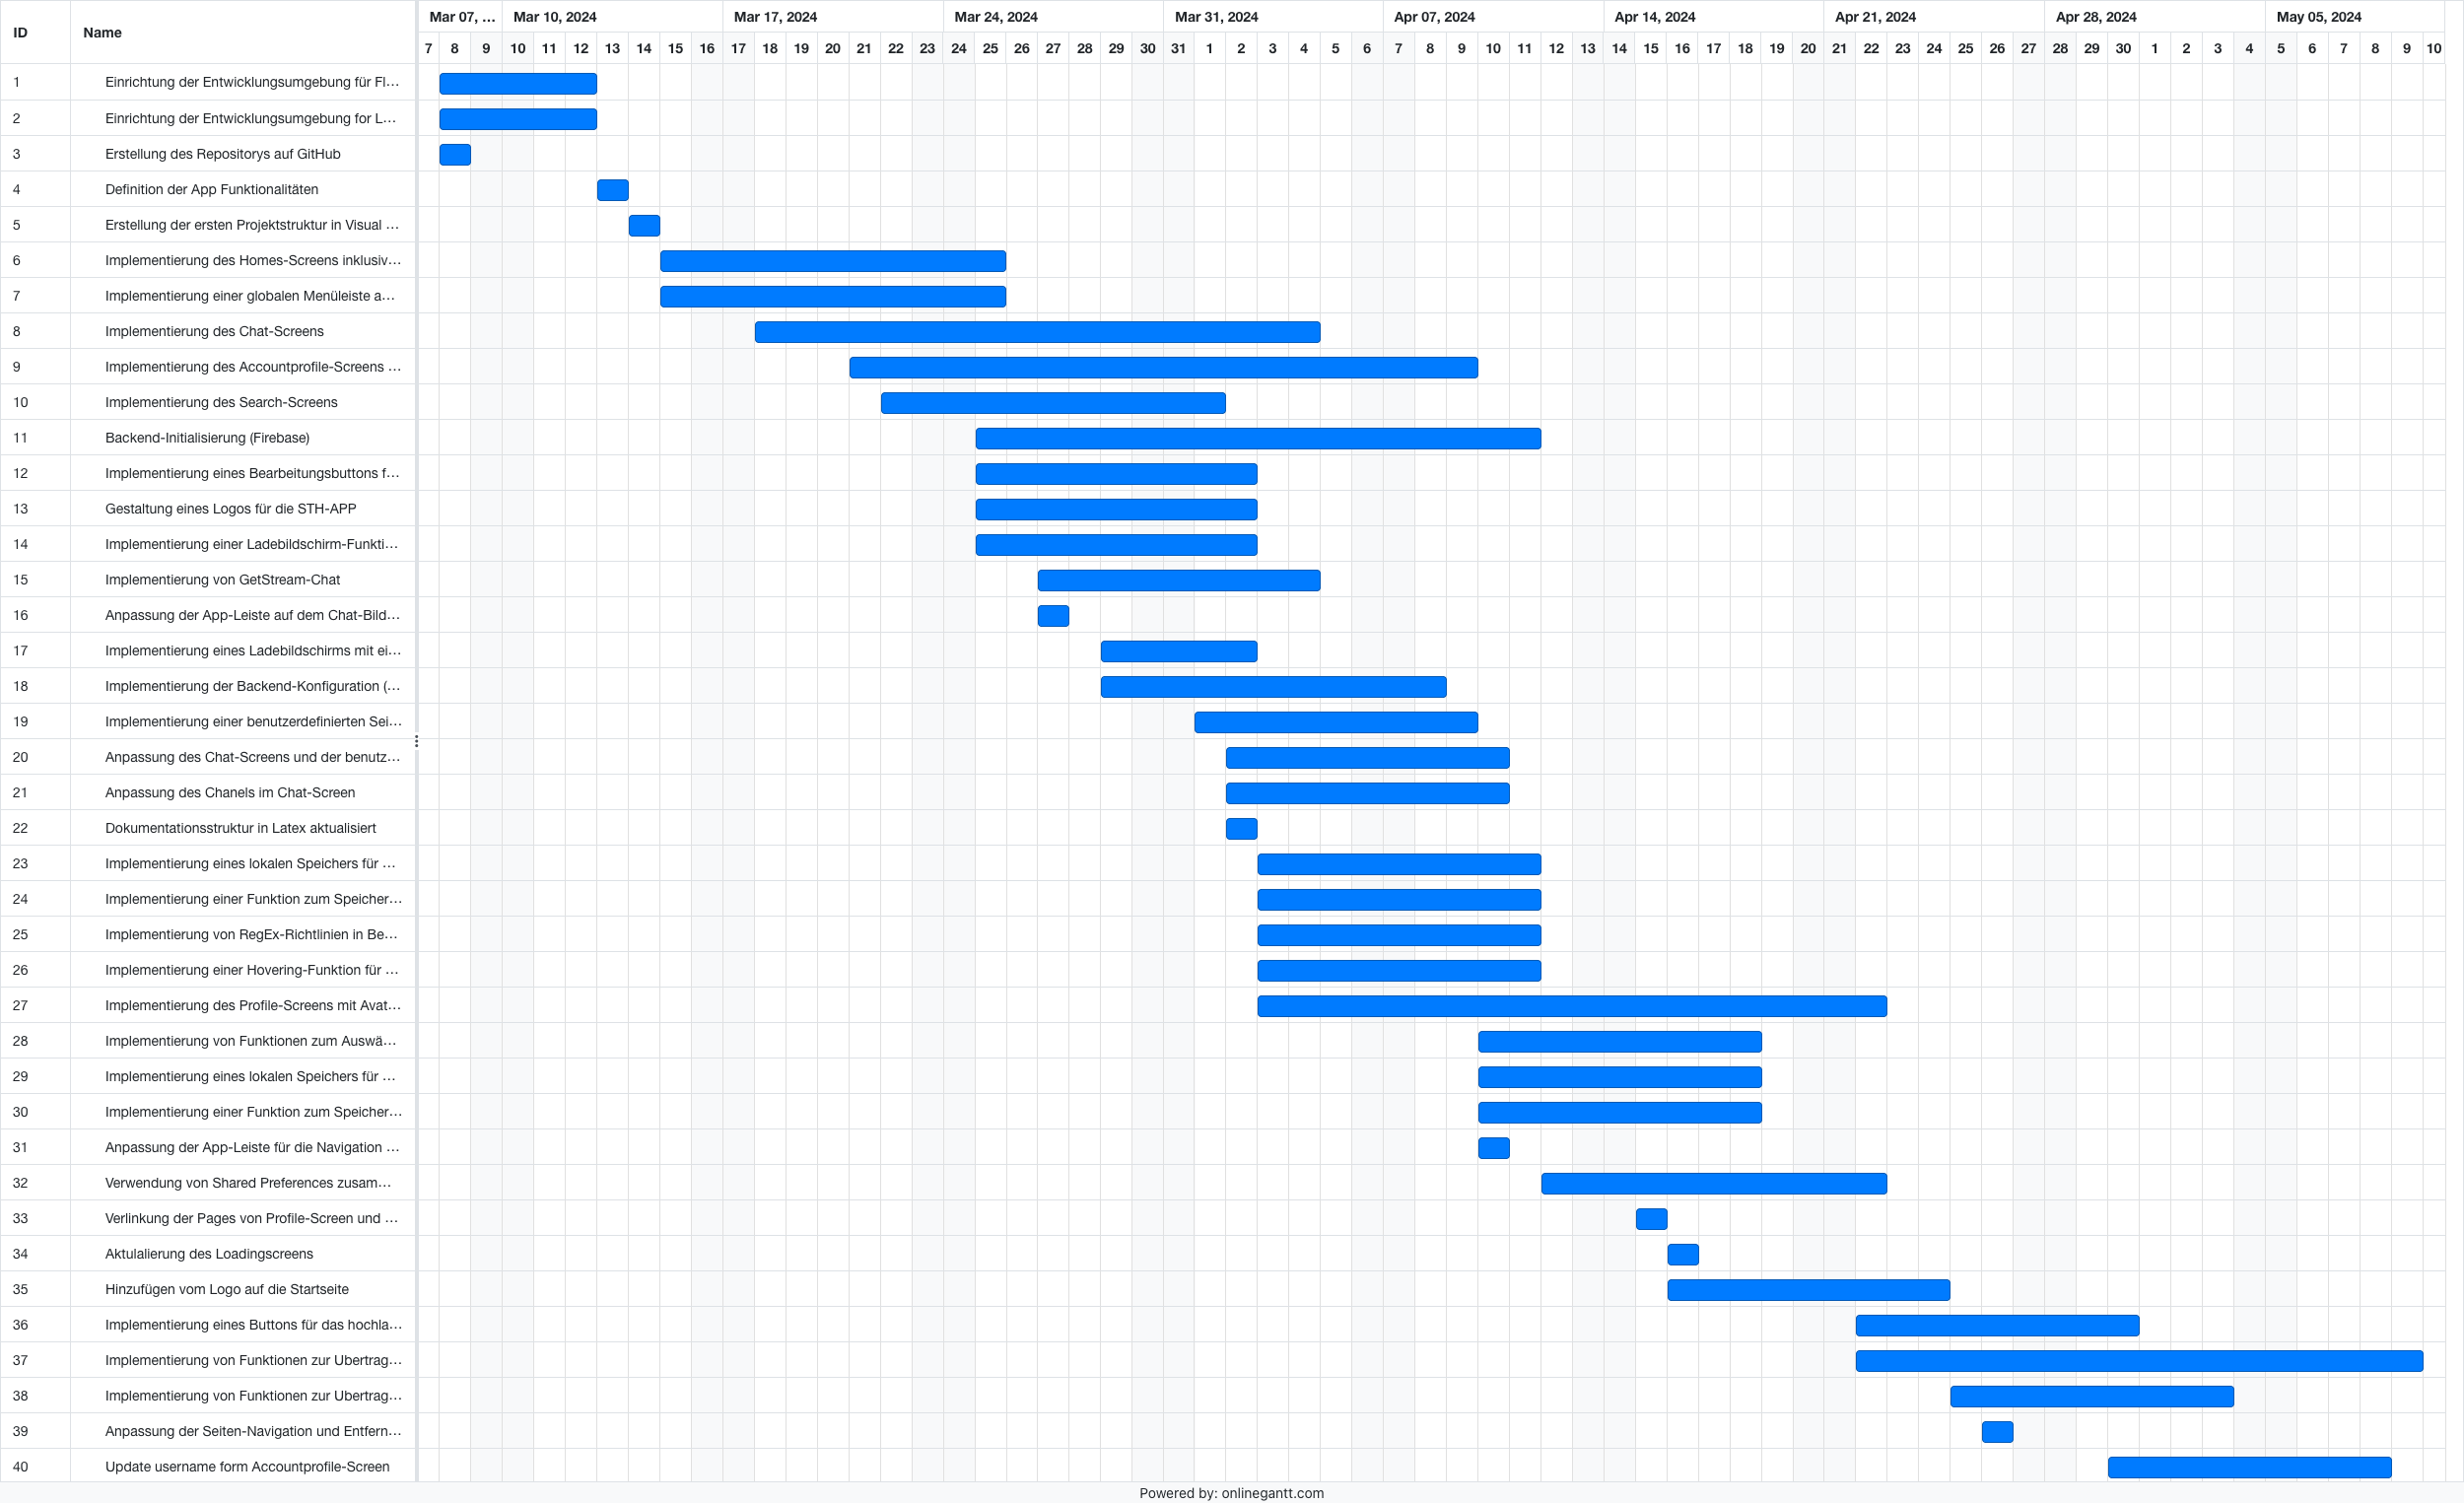
\includegraphics[width=0.9\textwidth]{assets/figures/STH GANTT Diagramm.png}
    \\
    Quelle: Test
\end{figure}

\chapter{Projektressourcen}
Im nächsten Schritt werden die Ressourcen beschrieben. Dazu zählen die am STH-App-Projekt beteiligten Personen und die materiellen Ressourcen.
Da es sich um ein Studienprojekt handelt, das die Entwicklung eines MVP einer App zum Ziel hatte, sind die aufgeführten Ressourcen speziell auf diesen Rahmen zugeschnitten.

\section{Personen}
\subsection{Projektteam}
Das Projektteam bestand aus vier Mitgliedern: Jonas Waigel, Fitim Makolli, Hasan Deveci und Vatsegkan Zournatsidis.
Jonas Waigel wurde als Projektleiter gewählt und war für die Koordination und Leitung des Teams verantwortlich.
Alle Teammitglieder brachten ihre individuellen Fähigkeiten und Erfahrungen ein, um gemeinsam die STH-App zu entwickeln.

\subsection{Personalaufwand}
Der Personalaufwand wurde in Personentagen gemessen. Da das Projekt über einen Zeitraum von vier Monaten lief, wurde der wöchentliche Aufwand pro Teammitglied auf etwa 10 Stunden geschätzt, was insgesamt 40 Stunden pro Woche für das gesamte Team ergibt. 
Über die Projektlaufzeit hinweg summiert sich dies auf etwa 2.560 Stunden (40 Stunden/Woche × 15 Wochen).


\subsection{Personalkosten}

\begin{itemize}
    \item \textbf{Jonas Waigel}
    \begin{itemize}
        \item \textbf{Stundensatz:} 120,00 €
        \item \textbf{Gesamtstunden:} 280 Stunden
        \item \textbf{Zeitraum:} 08.03.2024 - 18.06.2024
        \item \textbf{Gesamtkosten:} 33.600,00 €
    \end{itemize}

    \item \textbf{Fitim Makolli}
    \begin{itemize}
        \item \textbf{Stundensatz:} 110,00 €
        \item \textbf{Gesamtstunden:} 350 Stunden
        \item \textbf{Zeitraum:} 08.03.2024 - 18.06.2024
        \item \textbf{Gesamtkosten:} 38.500,00 €
    \end{itemize}

    \item \textbf{Hasan Deveci}
    \begin{itemize}
        \item \textbf{Stundensatz:} 130,00 €
        \item \textbf{Gesamtstunden:} 210 Stunden
        \item \textbf{Zeitraum:} 08.03.2024 - 18.06.2024
        \item \textbf{Gesamtkosten:} 27.300,00 €
    \end{itemize}

    \item \textbf{Vatsegkan Zournatsidis}
    \begin{itemize}
        \item \textbf{Stundensatz:} 150,00 €
        \item \textbf{Gesamtstunden:} 420 Stunden
        \item \textbf{Zeitraum:} 08.03.2024 - 18.06.2024
        \item \textbf{Gesamtkosten:} 63.000,00 €
    \end{itemize}
\end{itemize}

\textbf{Gesamtkosten:} 162.400,00 €

\section{Ressourcen}
\subsection{Ressourcenliste}
Die materiellen Ressourcen, die für die Entwicklung der STH-App erforderlich waren, umfassten:
\begin{itemize}
    \item Hardware: Laptops/Computer für jedes Teammitglied
    \item Software: Entwicklungsumgebungen (Visual Studio Code, xCode und Android Studio), Versionskontrollsystem (GitHub)
    \item Plattformen: Firebase für das Backend, Flutter für die plattformübergreifende App-Entwicklung
    \item Kommunikationstools: Microsoft Teams für die teaminterne Kommunikation und für regelmäßige Meetings und Stand-ups
    \item Testgeräte: Smartphones (iOS und Android) und Simulatoren / Emulatoren von xCode und Android Studio für Testzwecke
\end{itemize}

\subsection{Ressourcenkosten}

\begin{itemize}
    \item Hardware: 4 Laptops à 1200 € = 4800 €
    \item Software/ Entwicklungsumgebungen: Kostenfrei (durch Bildungsprogramme oder vorhandene Lizenzen)
    \item Plattformen: Firebase (kostenlose Nutzung innerhalb von bestimmten Grenzen), Flutter (kostenlos)
    \item Kommunikationstools: Microsoft Teams (kostenlose Nutzung für Bildungseinrichtungen)
    \item Testgeräte: Nutzung vorhandener Smartphones und kostenloser Simulatoren/Emulatoren
\end{itemize}

\noindent
Insgesamt wurden alle benötigten Ressourcen effizient genutzt, um die Entwicklung des MVP der STH-App ohne zusätzliche finanzielle Belastungen zu realisieren.
Dies ermöglichte es dem Team, sich vollständig auf die technischen, funktionalen und prozessualen Aspekte der App-Entwicklung sowie auf die Methoden des Projektmanagements zu konzentrieren und den Prototypen innerhalb des vorgegebenen Zeitrahmens erfolgreich umzusetzen.

\chapter{Initiale Einrichtung der Tools für das STH-Projekt}
Dieses Kapitel beschreibt die initiale Einrichtung des Flutter-Code-Repositories, die Nutzung von Google Firebase und die Verwendung vorhandener Microsoft Teams Add-On Tools für die Projektorganisation.

\section{Microsoft Teams Tools für die Organisation des Projektes und der Aufgaben für das Projektteam}
Im Projektstart-Meeting hat das Projektteam zusätzlich zur Ideenfindung und Projektteam-Aufteilung entschieden, dass das STH-Projekt mit agilen Projektmanagement-Methoden angelehnt an Scrum durchgeführt werden soll.
Zunächst wurde dafür ein Tool gesucht, das sowohl die Dokumentation von besprochenen Themen als auch die Planung von Aufgaben und die Kommunikation im Projektteam ermöglicht.
Nach einigen Recherechen und Diskussionen hat sich das Projektteam für Microsoft Teams entschieden.
Teams bietet mit seinen Add-On Tools die benötigten Möglichkeiten:\newline
Ergebnisse aus Diskussionen und Weekly-Standup-Meetings können mit Microsoft OneNote dokumentiert werden.
Aufgaben für das Projektteam können mit dem Add-On Microsoft Planner in einem Kanban Board übersichtlich dargestellt werden und der jeweilige Aufgabenstatus kann von jedem Projektmitglied eingesehen und bearbeitet werden.
Zusätzlich wurde ein Team in Microsoft Teams erstellt, in dem die Kommunikation im Projektteam stattgefunden hat und Neuerungen oder Probleme bei der Entwicklung besprochen werden konnten. 
\section{Einrichtung des Flutter-Code-Repositories für das STH-Projekt}
Im nächsten Schritt hat das Projektteam im Projektstart-Meeting ein Framework bzw\. eine Programmiersprache für das STH-Projekt gesucht, die sowohl eine gute Dokumentation, eine leicht verständliche Programmiersprache, Plattformunabhängigkeit für iOS/Android und die Kompatibilität zum Kompilieren der Applikation für die Betriebssysteme Windows und MacOS bietet.
Durch bereits vorhandenes Know-How wurde das Google-Framework Flutter gewählt.\newline
Flutter ist ein Open-Source-Framework von Google, das eine Frontend-Entwicklung von Benutzeroberflächen für Apps bietet.
Dabei gilt das Prinzip One-Codebase, welches bedeutet, dass Anwendungen für die unterschiedlichen Betriebssysteme iOS und Android aus einem Sourcecode kompiliert werden.
\newline
Für die Einrichtung des Repositories wird zunächst das Github Projekt ``anwendungsprojekt\_fom'' erstellt und das Projektteam freigegeben.
Im nächsten Schritt wurde auf den Entwicklungsrechnern der Projektmitglieder die Entwicklungsumgebung Visual Studio Code für die Code-Entwicklung und das Framework Flutter der Version 3\.19\.3 installiert und eingerichtet.
``Flutter'' bietet außerdem die Möglichkeit mithilfe des ``flutter create'' Terminal Commands ein initiales Flutter-Projekt erstellen zu lassen.
Dieses initiale Setup beinhaltet eine voll funktionsfähige Beispiel-App, die für den ersten Test des Setups erfolgreich für Android und iOS kompiliert werden konnte.
Für einen erfolgreichen iOS-Build wird zudem ein Apple-Gerät mit dem Betriebssystem macOS und die Apple-Software xCode benötigt, um iOS-spezifische Einheiten der App kompilieren zu können.
\newline
Für einen sogenannten ``Clean Code'', der für alle Projektmitglieder gut lesbar und verständlich ist, wurde festgelegt, dass für jede Änderung im Code der ``Flutter Formatter (Terminal Command: dart format -l 120 \.)\" und der Dart Analyzer (Terminal Command: dart analyze \&\& dart fix --apply)'' ausgeführt werden muss.
\section{Google Firebase Tools als Backend}
Firebase ist ein Cloud Service, der von Google bereitgestellt wird.
Dieser bietet folgende wichtige Funktionen, die für die STH App essentiell sind:
\begin{itemize}
    \item Der Cloud Firestore ist eine Cloud-Datenbank, in der verschiedene Werte von Variablen gespeichert werden können.
    \item Der Cloud Storage ist ein Cloud-Speicher, in dem Dateien unterschiedlicher Dateiformate hinterlegt werden können.
    \item Die Chat- und Kommunikationsfähigkeit
\end{itemize}
Über den Terminal\-Command ``flutter pub add'' incl\. den jeweiligen Flutter packages / dependencies \(firebase\_auth, firebase\_core, firebase\_storage, cloud\_firestore\) wurden Flutter Packages dem Projekt hinzugefügt und können verwendet werden.

\section{Zentrale Funktionen für Firebase, Shared Preferences, Flutter Page Routing, Flutter Bottom Navigationbar und Flutter App Bar}
Zusätzlich wurden Funktionen, die an anderen Stellen des Codes wiederverwendet werden, zentralisiert.
Dazu wurde im Repository ein Ordner ``technical'' angelegt und dieser in die jeweilige Grundfunktionalitäten unterteilt:
\\
\\
\textbf{Firebase}
\begin{itemize}[itemsep=0pt]
    \item{Authentifizierungsmethoden (Login / Register)} 
	\item{Datei-Upload und -Download Funktionen} 
	\item{Upload und Download von Variablenwerten} 
\end{itemize}
\textbf{Shared Preferences}
\begin{itemize}[itemsep=0pt]
    \item{Lokale Speicherung von Daten nach Download aus Firebase} 
	\item{Update Funktion von editierten Daten} 
\end{itemize}
\textbf{Custom Page Route}
\begin{itemize}[itemsep=0pt]
    \item{Einmalige zentrale Konfiguration des Routing-Verhaltens zwischen Screens} 
	\item{Flutter PageRouteBuilder incl\. generateRoute Funktion und neuer Screen als Übergabeparameter} 
\end{itemize}
\textbf{Custom App Bar}
\begin{itemize}[itemsep=0pt]
    \item{Einmalige zentrale Konfiguration der Flutter App Bar für ein einheitliches Design} 
	\item{Boolean-Übergabeparameter für die Anzeige von Buttons/Icons}
	\item{String-Übergabeparameter für den Seitentitel} 
\end{itemize}
\textbf{Custom Bottom Navigationbar}
\begin{itemize}[itemsep=0pt]
    \item{Einmalige zentrale Konfiguration der Flutter Bottom Navigationbar für ein einheitliches Design} 
	\item{Hervorhebung der aktuell ausgewählten Seite in der App}
	\item{Routing bei Auswahl eines Buttons in der Navigationbar} 
\end{itemize}


\chapter{Ladebildschirm}

Der Ladebildschirm ist ein essenzieller Bestandteil der Benutzererfahrung unserer STH-App (SportTalentHub). Er erscheint, bevor der Nutzer die Hauptfunktionen der App nutzen kann, und dient als Zwischenbildschirm, um dem Nutzer zu signalisieren, dass die App lädt.

\section*{Ziele des Ladebildschirms}
Der Ladebildschirm hat mehrere wichtige Funktionen. Er zeigt dem Nutzer visuelles Feedback, dass die App aktiv ist und lädt, wodurch eine bessere Benutzererfahrung gewährleistet wird. Der Ladebildschirm wurde so gestaltet, dass er genau vier Sekunden lang angezeigt wird. Dies gibt der App ausreichend Zeit, um die notwendigen Daten und Ressourcen im Hintergrund zu laden. \newline
Es ist entscheidend, dass nach Ablauf der vier Sekunden die Benutzer zur Startseite (Homepage) der App navigiert werden und nicht zu anderen Seiten wie der Profil- oder Chatseite.

\section*{Gestaltung des Ladebildschirms}
Für die Gestaltung des Ladebildschirms waren mehrere Schritte notwendig. Das Logo wurde mit Canva erstellt und musste den Charakter und die Zielgruppe der App widerspiegeln. \newline
Es wurde darauf geachtet, dass das Design für eine SportTalentHub-App geeignet ist. Die Inspiration für das Logo wurde aus verschiedenen Quellen, wie der NFL, gezogen. Die Farben und das Design sollten sportlich und ansprechend sein. \newline
Nach der Erstellung wurde das Logo transparent gemacht, um es optimal in den Ladebildschirm integrieren zu können.

Bevor das Logo endgültig in die App integriert wurde, wurde es im Rahmen eines wöchentlichen Meetings präsentiert. Das positive Feedback der Teammitglieder bestätigte die Eignung des Logos, sodass es anschließend in den Ladebildschirm eingefügt wurde.

Das Logo wurde im Ladebildschirm implementiert und ein animiertes Symbol hinzugefügt, das die Ladebewegung anzeigt. \newline
Es wurde darauf geachtet, dass nach dem Ablauf der vier Sekunden der Nutzer zur Startseite navigiert wird. Dies wurde durch entsprechende Programmierung in Flutter sichergestellt.

\section*{Änderungen am App-Logo}
Neben der Erstellung und Implementierung des Logos für den Ladebildschirm war es auch notwendig, das App-Logo selbst zu ändern. Das Ändern des App-Logos war technisch weniger anspruchsvoll. Es erforderte lediglich, das neue Logo in den entsprechenden Bereich des App-Projekts einzufügen. \newline
Wir entschieden uns außerdem, das Logo auch auf der Startseite der App anzuzeigen. Hierzu wurde ein Code in die Startseite geschrieben, der diese Funktion realisiert.

\chapter{Homescreen}
Der Homescreen ist der erste und damit wichtigste Anzeigebildschirm für die STH-App. 
Dieser wird direkt nach dem App Start angezeigt und ist somit sofort sichtbar.
\section*{Anforderungen an den Homescreen}
Für die Funktionalitäten auf dem Homescreen wurden zunächst vergleichbare Apps wie Instagram verglichen und die wichtigsten Funktionen ausgearbeitet.\newline
Folgende Anforderungen wurden dabei erstellt:\newline
- Profile/Posts von Sportlern anzeigen\newline
- Entry Point für die Chatfunktionalität

\section*{Erstellung der Flutter Widgets}
Zunächst hat der Homescreen die zentralen Elemente CustomAppBar und CustomNavigationBar erhalten.
Im nächsten Schritt wurde das sogenannte Post-Widget erstellt, das im Homescreen-Widget verwendet wird.
Grund dafür ist, dass die unterschiedlichen Posts der Sportler vom Grund-Designkonzept gleich aufgebaut sein sollen. 
Die Posts sollen sich nur durch die inhaltlichen / persönlichen Informationen unterscheiden.\newline
Aufgebaut ist ein Post mit einem Profilbild links oben, dem Profilnamen, den Bildern des Sportlerposts und einem Chat-Button, mit dem der Manager direkt zum jeweiligen Chat mit dem Sportler springt.

\section*{Daten aus Firebase für den Homescreen}
Die Informationen (Profilname) und Dateien (Bilder und Profilbild) für die Sportlerposts auf dem Homescreen werden aus Firebase geladen, indem die UserID der jeweiligen Sportler übergeben wird.
Aufgrund von Beispieldaten gibt es hier datenschutzrechtlich keine Einschränkungen, für einen möglichen Rollout der Funktionen in der App werden allerdings im Ausblick noch einige Verbesserungen / Möglichkeiten angesprochen.


\chapter{Suchbildschirm}

Der Suchbildschirm ist eine zentrale Funktion unserer STH-App (SportTalentHub). Er ermöglicht es den Nutzern, sowohl Sportlern als auch Sportmanagern, gezielt nach bestimmten Personen anhand von Hashtags oder Namen zu suchen.

\section{Ziele des Suchbildschirms}

Das Hauptziel des Suchbildschirms ist es, den Nutzern eine effiziente Möglichkeit zu bieten, Spieler oder Manager zu finden. Dies kann durch die Eingabe von Hashtags oder Namen erfolgen. Die Suchfunktion ist über das Suchsymbol auf dem Startbildschirm zugänglich.

\section{Integration mit Firebase}

Die Suchfunktion ist eng mit Firebase verbunden. Firebase spielt eine entscheidende Rolle, da dort die Profildaten der Nutzer gespeichert sind. Dadurch können Nutzer problemlos nach anderen Nutzern suchen. Wenn ein Suchbegriff, sei es ein Hashtag oder ein Name, eingegeben wird, erscheinen die gesuchten Personen auf dem Suchbildschirm. Bei Auswahl einer Person wird der Nutzer zu deren Profil weitergeleitet.

\section{Wichtigkeit der Suchfunktion}

Die Suchfunktion ist für unsere App von großer Bedeutung. Sie ermöglicht es Sportmanagern, gezielt nach bestimmten Merkmalen oder Fähigkeiten zu suchen und schnell und effektiv Ergebnisse zu erhalten. Dies verbessert die Benutzererfahrung und erhöht die Effizienz der App.

\section{Zukünftige Erweiterungen}

Zukünftige Erweiterungen der Suchfunktion könnten die Speicherung früher gesuchter Personen im Suchbereich umfassen. Außerdem wäre es möglich, die Suche zu erweitern, sodass nicht nur nach Hashtags und Namen gesucht werden kann, sondern auch nach weiteren Informationen oder Merkmalen.
\section{Profile-Screen \& Accountprofile-Screen}
In diesem Kapitel wird sowohl auf die Umsetzung der Flutter-Komponenten für den Profile-Screen als auch den Accountprofile-Screen des Projekts eingegangen.
Dabei liegt der Fokus auf die konzeptionelle Gestaltung und Implementierung beider App-Seiten, die es beispielsweise Benutzern ermöglichen, ihr Profilbild sowie multimediale Inhalte wie Bilder und Videos zu verwalten, aber auch personenbezogene Daten sicher abzuspeichern. 
Diese Funktionalitäten werden dabei unter Einsatz verschiedener Flutter-Pakete und Kernfunktionen der Dart-Programmiersprache umgesetzt. 
\\
Beginnend mit dem Profile-Screen, wird eine StatefulWidget-Klasse verwendet, die Zustandsänderungen verfolgt und das Benutzerinterface entsprechend aktualisiert.
Verschiedene Funktionen werden definiert, um auf Benutzerinteraktionen zu reagieren, beispielsweise das Öffnen von Galerieinhalten, das Laden von Bildern und Videos aus dem lokalen Speicher, das Hochladen von Medieninhalten auf Firebase sowie das Löschen von Bildern und Videos aus der Ansicht.
Darüber hinaus werden Methoden implementiert, um die Anwendungszustände zu verwalten, Benutzereingaben zu verarbeiten und Multimedia-Inhalte wie Bilder und Videos sicher zwischen dem lokalen Speicher, der in der Regel durch ``shared preferences'' verwaltet wird, und dem Backend in Firebase zu übertragen. 
Dadurch werden die Benutzerdaten effizient synchronisiert und sicher in der Cloud gespeichert, wodurch Datenschutz und Datensicherheit gewährleistet werden. 
Bei Bedarf können diese Daten dann abgerufen und aktualisiert werden. Dabei spielen bei der Implementierung dieser Features folgende Methoden eine entscheidende Rolle:
\\``build'' ist die Methode, die das Benutzerinterface basierend auf dem aktuellen Zustand der StatefulWidget-Klasse aufbaut. Sie ist der Ausgangspunkt für den Aufbau der UI-Elemente und ermöglicht die dynamische Erstellung und Aktualisierung des Bildschirms. 
Die Methode ``initState'' spielt eine wichtige Rolle bei der Initialisierung des Zustands der StatefulWidget-Klasse. Hier werden unter anderem Informationen aus dem lokalen Speicher geladen und andere vorbereitende Maßnahmen getroffen, um das Benutzerinterface entsprechend anzupassen und eine konsistente Benutzererfahrung zu gewährleisten. 
Diese beiden Methoden bilden das Rückgrat des Profile-Screens und ermöglichen es, mithilfe von weiteren Methoden, die Benutzeroberfläche zu strukturieren und den Zustand der App zu verwalten.
Zusätzliche Methoden wie ``openGallery'' und ``openVideo'' sind von entscheidender Bedeutung, um dem Benutzer die Möglichkeit zu geben, Bilder und Videos auszuwählen und anzuzeigen. 
Durch das Öffnen neuer Bildschirmfenster bieten sie eine intuitive Benutzeroberfläche und ermöglichen es dem Benutzer, Inhalte zu erkunden. 
Darüber hinaus bieten sie Funktionen zum Anzeigen, Schließen und Löschen von Inhalten, was die Interaktivität und Benutzerfreundlichkeit der STH-App verbessert.
Methoden wie ``loadAvatarImage'' und ``loadUserName'' spielen eine essenzielle Rolle, um den Avatar des Benutzers und seinen Benutzernamen aus dem lokalen Speicher zu laden. 
Diese Informationen werden wiederum aus dem Accountprofile-Screen bezogen, was eine Integration und eine personalisierte Anpassung des Benutzerinterfaces ermöglicht. 
Durch das Laden dieser Daten können Benutzer ihre Profile individuell gestalten und ein konsistentes Benutzererlebnis über verschiedene Bildschirme hinweg gewährleisten. 
Im Kontext der Datenschutzsicherheit spielen Methoden wie ``saveImagePathsToLocalStorage'', ``saveImage'', ``loadImagesFromStorage'' und ``uploadGalleryImages'' eine entscheidende Rolle beim Speichern, Laden und Hochladen von Bildern. 
Diese Methoden ermöglichen es Benutzern, ihre Bilder sowohl lokal im lokalen Speicher über die SharedPreferences als auch in der Cloud über das Backend in Firebase sicher zu verwalten und zu teilen. 
Durch die Verwendung dieser Methoden wird die Integrität der Benutzerdaten gewahrt und gleichzeitig eine zuverlässige Speicherung und Übertragung von Bildinhalten gewährleistet. 
Ähnlich wichtig sind Methoden wie ``saveVideoPathsToLocalStorage'', ``saveVideo'', ``loadVideosFromStorage'' und ``uploadVideos'' für die Verwaltung von Videos.
Sie ermöglichen es dem Benutzer, multimediale Inhalte zu verwalten und zu teilen. Dabei werden die Videodaten sowohl lokal im lokalen Speicher gespeichert als auch über das Backend in Firebase hochgeladen, wo sie für weitere Verwendungszwecke verfügbar sind.
Diese Methoden spielen somit eine essenzielle Rolle bei der Sicherung und Bereitstellung von Videoinhalten für die Benutzer der App.
Um dem Benutzer die Kontrolle über seine Inhalte zu geben, dienen ``deleteImage'' und ``deleteVideo'' dazu, ausgewählte Bilder und Videos zu löschen. 
``generateThumbnail'' ermöglicht es, Vorschaubilder für Videos anzuzeigen, um dem Benutzer eine Vorschau des Inhalts zu bieten.
Die Methoden ``saveHashtagsToLocalStorage'', ``loadHashtagsFromStorage'' und ``deleteHashtagFromLocalStorage'' tragen zur Verwaltung von Hashtags bei und verbessern die Personalisierung und Relevanz der bereitgestellten Inhalte. 
Die Methode ``showHashtagsModal'' erlaubt es dem Benutzer, Hashtags auszuwählen und hinzuzufügen, um seine Interessen zu kennzeichnen. Sie fördert die Benutzerbeteiligung und ermöglicht die Personalisierung von Inhalten.
Die Benutzeroberfläche des Profilbildschirms setzt sich aus einem Header-Bereich mit dem Benutzernamen und dem Profilbild sowie einem Abschnitt zur Anzeige und Verwaltung von Bild- und Videoinhalten zusammen. 
Die Anzeige kann zwischen Bildern und Videos umgeschaltet werden, und Benutzer haben die Möglichkeit, neue Medieninhalte auszuwählen und hochzuladen, welche von den Methoden pickMultiImage und pickVideo unterstützt werden. 
Für die Gestaltung der Benutzeroberfläche kommen verschiedene Flutter-Widgets wie Column, Stack, AppBar, CircleAvatar und GridView zum Einsatz, um eine ansprechende und benutzerfreundliche Erfahrung zu gewährleisten.
Zusätzlich werden benutzerdefinierte Widgets wie CustomAppBar und CustomBottomNavigationBar verwendet, um die Navigation und Interaktion zu erleichtern und das Design konsistent zu halten.
\\
Im Accountprofile-Screen hingegen erscheinen bearbeitbare personenbezogene Daten, wobei zur Validierung der Eingaben reguläre Ausdrücke (Regex) herangezogen werden. 
Den Nutzern wird die Gelegenheit geboten, ihre Profildaten anzupassen und zu sichern – darunter fallen der Name, die Telefonnummer, die Adresse und die E-Mail-Adresse. 
Beim Start des Bildschirms werden die aktuellen Profildaten aus den SharedPreferences geladen und in entsprechenden Textfeldern angezeigt. 
Nutzer können diese Informationen bearbeiten und die Änderungen anschließend speichern. Hier haben Nutzer die Freiheit, ein Profilbild zu wählen, das dann in einem kreisförmigen Avatar angezeigt wird. 
Das ausgesuchte Bild wird nicht nur lokal auf dem Gerät gespeichert, sondern auch im Backend abgelegt. Bei Bedarf wird es von Firebase abgerufen, um anderen Seiten mit den entsprechenden Daten zu bereichern. Die Benutzeroberfläche des Accountprofilbildschirms besteht aus mehreren Textfeldern für die Bearbeitung von Profildaten sowie einem Abschnitt für das Profilbild. 
Im Bearbeitungsmodus werden die Textfelder kenntlich und sichtbar zur Bearbeitung hervorgehoben, sodass Nutzer ihre Daten ändern können. Fehlermeldungen erscheinen, falls ungültige Eingaben gemacht wurden, und ein Tooltip mit einem Hover-Effekt informiert die Nutzer über die Art des Fehlers.
Auch hierbei wurden folgende Methode zur Implementierung benötigt, um unseren konzeptionellen Anforderungen gerecht zu werden.
\\
Die Build-Methode erstellt die Benutzeroberfläche des Accountprofil-Screens. Sie umfasst Textfelder für die Bearbeitung von Profildaten sowie einen Bereich für das Profilbild. 
Die UI wird je nach Bearbeitungsstatus der Daten dynamisch angepasst. Die PickImage-Methode ermöglicht es Benutzern, ein Profilbild auszuwählen und es hochzuladen. Sie wird aktiviert, sobald der Benutzer auf die entsprechende Schaltfläche klickt.
Dadurch wird die Bildauswahl gestartet, und das ausgewählte Bild wird für das Profil verwendet. Beim Start des Bildschirms ruft die LoadProfileData-Methode die aktuellen Profildaten aus den SharedPreferences ab. 
Diese Daten, einschließlich Name, Telefonnummer, Adresse und E-Mail, werden dann in den entsprechenden Textfeldern angezeigt, damit der Benutzer sie bearbeiten kann. Um das ausgewählte Profilbild lokal zu speichern und sicherzustellen, dass es für spätere Verwendungszwecke verfügbar ist, wird die Methode saveAvatarImage verwendet.
Nachdem der Benutzer ein Bild ausgewählt hat, wird es lokal auf dem Gerät gespeichert. Zusätzlich dazu werden die aktualisierten Profildaten, einschließlich des Profilbildes, im Backend gespeichert, damit das Profilbild auch von anderen Seiten oder Anwendungen wiederverwendet werden kann. 
Die LoadAvatarImage-Methode wird aufgerufen, um das Profilbild aus der lokalen Speicherung zu laden. Dadurch wird das zuvor gespeicherte Profilbild beim Öffnen des Accountprofil-Screens geladen und im Kreisavatar angezeigt. 
Für die Validierung der personenbezogenen Daten werden unter Verwendung von regulären Ausdrücken (Regex) folgende Methoden verwendet. Diese dienen dazu, sicherzustellen, dass die eingegebenen Daten gültig sind, bevor sie gespeichert werden. Dabei werden sämtliche personenbezogenen Daten sowohl lokal auf dem Gerät als auch im Backend gespeichert, um die Integrität der Daten zu gewährleisten und sicherzustellen, dass sie für verschiedene Anwendungen verfügbar sind: 

\begin{itemize}[itemsep=0pt]
    \item{Die ValidatePhone-Methode validiert die eingegebene Telefonnummer und akzeptiert nur Zahlen und optional ein Pluszeichen am Anfang}
\end{itemize}
\begin{itemize}[itemsep=0pt]
    \item{Um die Gültigkeit der eingegebenen Adresse zu überprüfen, wird die ValidateAddress-Methode verwendet. Diese erwartet Buchstaben, Zahlen, Kommas, Punkte, Leerzeichen und Umlaute als gültige Zeichen} 
\end{itemize}
\begin{itemize}[itemsep=0pt]
	\item{Die ValidateEmail-Methode prüft, ob die eingegebene E-Mail-Adresse gültig ist und erwartet das übliche Format einer E-Mail-Adresse}
\end{itemize}
Während des abschließenden Bearbeitungsvorgangs wird die Methode updateUserData aufgerufen. Diese Funktion dient dazu, die Profildaten in der Cloud Firestore-Datenbank zu aktualisieren. Dabei werden sämtliche neuen Informationen wie Name, Telefonnummer, Adresse und E-Mail in der Datenbank aktualisiert, um sicherzustellen, dass sie synchronisiert und auf dem neuesten Stand sind. Dies ermöglicht es, die aktualisierten Daten für andere Zwecke zu beziehen und weiterzuverwenden. Sobald der Benutzer die Profildaten bearbeitet hat, werden diese mithilfe der SaveProfile-Methode in den SharedPreferences gespeichert, um sie beim nächsten Öffnen des Bildschirms wiederherzustellen.  Die Interaktion zwischen dem Profilbildschirm und dem Accountprofilbildschirm sowie der Datenaustausch zwischen ihnen bestimmen die grundlegende Ausrichtung der App-spezifischen Funktionen. Diese Funktionen erstrecken sich auf verschiedene Bereiche der Anwendung, wie beispielsweise den Home-Screen über das Backend, die dem Benutzer die Wiedergabe von Informationen in Form von Bildern, Videos und personenbezogenen Daten ermöglicht. Auch der Suchbildschirm profitiert von der Implementierung der Daten über das Backend, da dieser den Suchalgorithmus unterstützt und dem Benutzer dabei hilft, relevante Ergebnisse zu finden, die im Sinne einer Social-Media-App agieren.



\section{Implementierung des Chat-Screens}
Zu jeder modernen Community Applikation gehört auch die Chatfunktionalität dazu. Der Austausch zwischen zwei oder mehreren Menschen ist besonders in der STH-App wichtig, um die Kommunikation zwischen Spielern und Managern zu ermöglichen. Die Anforderungen an den Chat-Screen standen schnell fest. Die Funktionalität muss mindestens den gleichen Interaktionsumfang ermöglichen, wie vergleichbare Apps wie z.B. Instagram, Snapchat oder X (ehemalig Twitter).

\subsection{Anforderungen an den Chat-Screen}
Die spezifischen Anforderungen für die Chat-Funktion in der STH-App wurden im Projektteam gemeinsam ausgearbeitet. Dabei wurden zunächst vergleichbare Applikationen genauer beleuchtet und die Mindestanforderungen anhand der dort gesichteten Funktionen definiert. Das Chatten in der STH-App muss mittels verschlüsselte eins zu eins Verbindungen funktionieren, in der zwei Menschen miteinander in einem Chat-Raum kommunizieren können. Zudem muss es auch die Möglichkeit geben Gruppenchats zu erstellen und mehrere Menschen dazu einzuladen. Auch hierbei müssen die Verbindungen stets verschlüsselt sein. Innerhalb eines Chats muss jeder Nutzer Nachrichten senden und empfangen können. Zu den Nachrichten gehören Textnachrichten, GIFs, Bilder und Videos. Jeder Nutzer muss gesendete und empfangene Nachrichten im Chat sehen können und die Chats müssen mit ihrem kompletten Verlauf beim ein- und ausloggen erhalten und neu geladen werden können.

\subsection{Erstellung einer Flutter Widget-Seite}
Nachdem die Anforderungen definiert wurden, kann nun die Erstellung der Chat-Screen Widget-Seite beginnen. Diese Seiten dienen als Vorbereitung dazu, Widgets platzieren und anzeigen zu können. Das Erstellen einer derartigen Seite kann in Flutter durch das Erstellen einer Klasse realisiert werden. Hierbei wird für die Klasse ein kontextbezogener Name eingesetzt und die Art der Widget-Seite definiert. Dabei wird zwischen Stateful und Stateless Widgets unterschieden. Bei den Stateful Widget Klassen können sich deren Komponenten verändern. Die Stateless Widgets verändern sich nicht und können sich nicht in der Ansicht aktualisieren. Für den Chat-Screen ist das Stateful Klassenwidget die richtige Wahl, da sich die Anzahl und Inhalte der angezeigten Chats stetig verändern kann.

\subsection{Integration des Stream-Chat-Flutter Pakets}
Die Implementierung einer Chat-Funktion kommt in Social-Media Apps sehr häufig bzw. fast immer vor. Deshalb gibt es hierzu eine große Anzahl an Flutter Paketen, welche sich unter der Seite pub.dev genauer angeschaut werden können. Ein sehr mächtiges und umfängliches Paket nennt sich hierbei Stream-Chat-Flutter. Dieses Paket bringt eine Anzahl an vorbereiteten Widgets für die Anzeige und Erstellung von Chats mit sich. Darin beinhaltet sind App-Bars, Channel-Screens, Chat-Screens und Chatfunktionen. Die Einbindung dieses Pakets erfordert das Verändern der gesamten Struktur der Anwendung. Die Chat-Funktion stellt einen Hauptbestandteil der Anwendung dar und muss auf den Top of Widget-Tree implementiert werden. Das bedeutet, dass das Paket Stream-Chat-Flutter als Erstes in der Anwendung geladen werden muss, um es korrekt auszuführen. Nachdem die Struktur und das Laden der Pakete in der Anwendung angepasst wird, müssen Funktionen implementiert werden, die das Abrufen von Chats aus dem Stream-Chat-Client ermöglichen. Dabei greift die STH-App auf das separate Backend des Paketes zu und authentifiziert den aktuellen Nutzer der Applikation. Nach erfolgreicher Authentifizierung werden die zugehörigen Chatdaten und Channels abgerufen, um dem Nutzer alle Chatverläufe korrekt anzeigen zu können.

\subsection{Benutzerauthentifizierung}
Um die Benutzerauthentifizierung durch die Anwendung zu ermöglichen, müssen Zugangsschlüssel bzw. Tokens bereitstehen. Diese Tokens werden durch den Aufruf durch Firebase generiert und der jeweilige Nutzer der Anwendung registriert. Nach erfolgreicher Übermittlung der Tokens kann die STH-App nun sicherstellen, dass es sich um den angemeldeten Nutzer handelt und alle Chatverläufe inklusive persönliche Daten laden. 

\subsection{Implementierung der Chat-Widgets}
Nach der erfolgreichen Benutzerauthentifizierung folgt der letzte Schritt. Die verschiedenen Chats des Nutzers und die Chatverläufe können mittels der Chat-Widgets aus dem Paket Stream-Chat-Flutter angezeigt werden. Das Paket beinhaltet einen vollständigen Channel-Screens. Das ist das Widget, welches zuerst beim Einstieg in die Chat-Funktionen angezeigt wird. Analog zu anderen bekannten Applikationen wird hierbei eine Übersicht über alle aktiven Chats des Nutzers angezeigt. Daraufhin folgt der Channel-Screen. Dieser stellt den einzelnen Chat, auf dem vom Channel-Screen aus geklickt wird, dar. Im Chat-Screen ist der gesamte Chatverlauf aus diesem Chat des Nutzers zu sehen. Zudem kann hier durch das Textfeld am unteren Ende der Seite neue Nachrichten durch den Nutzer eingegeben werden und an den Chatpartner versendet werden.

\noindent
Die Implementierung des Channel-Screens erfolgt als Erstes. Hierfür wird eine eigene Klasse erstellt und das Chat-Screen Widget aus dem Paket wird auf dieser Seite platziert. Nun muss noch das richtige Routing definiert werden. Das stellt sicher, dass die verschiedenen Chats geladen werden können. Die Liste der verfügbaren Chats wird geladen und am oberen Ende der Seite wird die App-Bar mit dem Namen Chats angezeigt.

\noindent
Nach der Integration des Channel-Screen-Widgets kann nun das Chat-Screen-Widget folgen. Für das Chat-Screen-Widget wird ebenso eine neue Klasse und Seite erstellt, worauf das Widget platziert werden kann. Nach der Platzierung wird durch das korrekte Routing sichergestellt, dass der richtige Chat vom angemeldeten User geöffnet wird. Durch die Integration des Paketes sind alle Funktionen automatisch verfügbar. Das Versenden und Empfangen von Nachrichten ist bereits möglich und das Reagieren auf Nachrichten ebenso. Zu normalen Textnachrichten können auch Bilder, GIFs, Videos und Emojis versendet werden. Die Grundfunktionalitäten einer ausgereiften Social-Media App stehen nun mit der Chat-Funktion.

\noindent
Nun ist der letzte Schritt die Anwendung auf die korrekte Wegweisung bzw. Routing anzulernen. Dabei wird in der main.dart, welches die Hauptdatei darstellt und dabei auch die Strukturen für die gesamte Anwendung festlegt, das Routing eingearbeitet. Die neuen Screens müssen den gesamten Routing Optionen der Anwendung hinzugefügt werden. Die dabei verwendeten Klassen werden referenziert. Innerhalb der Datei CustomAppBar wird nun für den Chat-Button das korrekte Routing hinterlegt. Dabei wird auch festgelegt, in welchen Bildschirmen der Chat-Button sichtbar ist und in welchen nicht. Innerhalb des Chat-Screens verschwindet der Chat-Button, da der Anwender sich bereits in der Chatfunktionalität aufhält. In allen anderen Ansichten ist der Button sichtbar und das Routing erfolgt beim Auslösen. Nun ist der Channel-Screen und der Chat-Screen in der Anwendung vollständig mit korrektem Routing implementiert.

\chapter{Fazit}
Im Rückblick auf das Projekt STH-App lässt sich festhalten, dass die zu Projektbeginn definitierten Ziele erreicht wurden.
Die STH-App schafft nun eine innovative Lösung, Sportmanager und Sportler über die Chat-Funktion miteinander kommunizieren zu lassen.
Zudem gewährleistet das genutzte Framework Flutter die Plattformunabhängigkeit zwischen Apple iOS Geräten und Android Geräten und zusätzlich die Aktualität durch regelmäßige Updates.
Das Design wurde speziell für die STH-App entwickelt und zeigt Konsistenz und eine gute User Experience mithilfe von aussagekräftigen Icons.
Des Weiteren wurde die Integration der Google Firebase Tools und vor allem die sofortige Datenübertragung als gelungen betrachtet.\newline
Für diesen aktuellen Stand der App war vor allem die sehr enge Zusammenarbeit der Teammitglieder und der Einsatz von modernen Tools ausschlaggebend.
Speziell die wöchentlichen strukturierten Besprechungen der aktuellen Fortschritte und Probleme der Teammitglieder, aber auch die weitere Planung haben sehr geholfen, den aktuellen Stand des Projektes zu erreichen.
Während des Projektes sind mithilfe der manuellen kontinuierlichen App-Tests bei der Entwicklung neuer Funktionen von den Teammitgliedern regelmäßig Bugs und Verbesserungsvorschläge gefunden, die während den Weekly-Standups dokumentiert und dementsprechend eine neue Aufgabe im Teamboard erstellt wurde.\newline
Trotz anfänglicher technischer Schwierigkeiten beim Einrichten der Entwicklungsumgebungen auf den unterschiedlichen Betriebssystemen, Kompilierfehler durch Änderungen am Sourcecode und Verzögerungen bei der Entwicklung wurden dennoch alle gesetzten Meilensteine erreicht.
Langfristig kann die STH-App vor allem durch die einfache und zuverlässige Architektur und die Benutzerfreundlichkeit ein großes Potential in verschiedenen Märkten erreichen.\newline
Während des Projekts konnten wir wertvolle Erfahrungen sammeln, insbesondere in Bezug auf die agile Arbeitsweise und die Nutzung von Tools zur Zusammenarbeit.
Ein entscheidender Erfolgsfaktor war auch das offene Feedback und die kontinuierliche Verbesserung basierend auf den Ergebnissen der App-Tests.

\chapter{Ausblick}

Mit Blick auf die zukünftige Entwicklung der STH-App sind mehrere bedeutende Erweiterungen und Verbesserungen geplant, um die App kontinuierlich zu optimieren und das Benutzererlebnis zu verbessern:

\begin{itemize}
\item Verbesserung des Suchalgorithmus für den Search-Screen: Die Optimierung des Suchalgorithmus wird die Effizienz und Genauigkeit der Suchergebnisse erhöhen, wodurch Nutzer schneller und präziser die gewünschten Informationen finden können.
\item Verbesserung der UI/UX-Implementierung: Ein überarbeitetes und schöneres Design steigert die Benutzerfreundlichkeit der App weiter, was zu einer intuitiveren und angenehmeren Benutzererfahrung führt. Dabei kann die Bedienung der App durch gezielte Anpassungen bestehender Funktionen weiter vereinfacht und die Zufriedenheit der Nutzer erhöht werden.
\item Einrichten von In-App-Linkouts für einen direkten Wechsel zu einem anderen Screen: Diese Funktion ermöglicht es Nutzern, direkt zwischen verschiedenen Bildschirmen zu wechseln, was das Navigieren innerhalb der App verbessert.
\item Integration von KI-basierten Features: Durch den Einsatz von künstlicher Intelligenz können personalisierte Empfehlungen und automatisierte Prozesse erzeugt werden, die das Nutzererlebnis noch individueller und effizienter gestalten. Die KI-Features können beispielsweise auf dem Home-Screen oder Search-Screen bei der Suche von Sportlern oder Sportmanagern helfen.
\item Lokalisierung und Übersetzungen von Texten in der App: Die Lokalisierung und Übersetzung der App-Inhalte in verschiedene Sprachen wird die Reichweite der STH-App erweitern und die Benutzerfreundlichkeit für internationale Nutzer erhöhen.
\item Implementierung von Personalisierungsoptionen: Nutzern werden mehr Möglichkeiten zur individuellen Anpassung der App geboten, was deren Engagement und Zufriedenheit fördern wird.
\end{itemize}
Zusätzlich sollen auch technische Versionsupdates des Frameworks Flutter, der dazugehörigen Dependencies sowie von Apple und Google berücksichtigt und der Source-Code der STH-App dementsprechend aktualisiert werden. Dies stellt sicher, dass die App immer auf dem aktuellen Stand der Technik bleibt und optimale Performance bietet.
Weitere wichtige Punkte sind die Performance der STH-App auf den Geräten der Nutzer sowie die Sicherheit und der Datenschutz. 
Mögliche Herausforderungen, wie die Anpassung an verschiedene regionale Anforderungen, werden durch gezielte Forschung und Entwicklung adressiert.
In den kommenden Monaten wird das Projektteam verstärkt auf Innovationsprozesse und Marktanalysen setzen, um die App kontinuierlich zu optimieren und das Benutzererlebnis zu verbessern. Dabei wird eine umfassende Teststrategie entwickelt, die verschiedene Testmethoden wie UI-Tests, A/B-Tests, manuelle Tests, Testautomatisierung, Unit-Tests und Crowdtests umfasst. Dies dient dazu, Benutzerwünsche und -feedback gezielt zu erfassen und ein breites Spektrum an Nutzern zu berücksichtigen.
Langfristig plant das Projektteam die Veröffentlichung der STH-App inklusive Wartung und technischem Support. Eine Community beziehungsweise ein Forum soll aufgebaut werden, um kontinuierliches Feedback zu erhalten und regelmäßige Fehlerbehebungen sowie Verbesserungen über App-Updates umzusetzen.\newline
Abschließend lässt sich feststellen, dass dieses Projekt in der Zukunft zahlreiche Möglichkeiten und Optionen für den Erfolg der STH-App bietet. Durch die geplanten Erweiterungen und die konsequente Ausrichtung auf die Bedürfnisse der Nutzer wird die STH-App ihre Position als innovatives und nützliches Werkzeug für Sportmanager und Sportler weiter festigen und ausbauen.

\input{erklärung.tex}

\pagenumbering{gobble}

%end of document
\end{document}
